%%%%%%%%%%%%%%%%%%%%%%%%%%%%%%%%%%%%%%%%%%%%%%%%%%%%%%%%%%%%%%%%%%%%%%%%%%%%%%%%%%
\begin{frame}[fragile]\frametitle{}
\begin{center}
{\Large Demonstration Skills}
\end{center}
\end{frame}

%%%%%%%%%%%%%%%%%%%%%%%%%%%%%%%%%%%%%%%%%%%%%%%%%%%%%%%%%%%
\begin{frame}[fragile]\frametitle{Syllabus}

\begin{itemize}
\item 4.1  Prayer: Concept and recitation of \textit{Pranava} (\textit{प्रणव}) and hymns. 
\item 4.2  Yoga Cleansing Techniques: Knowledge of Dhauti (\textit{धौती}), Neti (\textit{नेति}) and practice of Kapalabhati (\textit{कपालभाति}). 
\item 4.3  Yogic Sukshma Vyayama (\textit{सुक्ष्म व्यायाम}) and Sthula Vyayama (\textit{स्थूल व्यायाम})      
	\begin{itemize}
	\item a. Yogic Sukshma Vyayama (Micro Circulation Practices) 
		\begin{itemize}
		\item Neck Movement: Griva Shakti Vikasaka (\textit{ग्रीवा शक्ति विकासक}) (I, II, III, IV) 
		\item Shoulder Movement: Bhuja Valli Shakti Vikasaka (\textit{भुजा वल्ली शक्ति विकासक}), Purna Bhuja Shakti Vikasaka (\textit{पूर्ण भुजा शक्ति विकासक}) 
		\item Trunk Movement: Kati Shakti Vikasaka (\textit{कटि शक्ति विकासक}) (I, II, III, IV, V) 
		\item Knee Movement: Jangha Shakti Vikasaka (\textit{जङ्घा शक्ति विकासक}) (II-A \& B), Janu Shakti Vikasaka (\textit{जानु शक्ति विकासक})
		\item Ankle Movement: Pada-mula Shakti Vikasaka (\textit{पाद-मूल शक्ति विकासक}) – A \& B, Gulpha-pada-pristha-pada-tala Shakti Vikasaka (\textit{गुल्फ-पाद-पृष्ठ-पाद-तल शक्ति विकासक})
		\end{itemize}
	\item b. Yogic Sthula Vyayama (Macro Circulation Practices) 
		\begin{itemize}
		\item Sarvanga Pushti (\textit{सर्वाङ्ग पुष्टि})
		\item Hrid Gati (\textit{हृद् गति}) (Engine Daud)
		\end{itemize}
	\end{itemize}
\end{itemize}
\end{frame}


%%%%%%%%%%%%%%%%%%%%%%%%%%%%%%%%%%%%%%%%%%%%%%%%%%%%%%%%%%%
\begin{frame}[fragile]\frametitle{Syllabus}

\begin{itemize}
\item 4.4  Yogic Surya Namaskara (\textit{योगिक सूर्य नमस्कार})   
\item 4.5  Yogasana (\textit{योगासन}) 
	\begin{itemize}
	\item Tadasana (\textit{ताड़ासन}), Vrikshasana (\textit{वृक्षासन}), Ardha Chakrasana (\textit{अर्ध चक्रासन}), Padahastasana (\textit{पादहस्तासन}), Kati Chakrasana (\textit{कटिचक्रासन}), Trikonasana (\textit{त्रिकोणासन})  
	\item Dandasana (\textit{दंडासन}), Sukhasana (\textit{सुखासन}), Padmasana (\textit{पद्मासन}), Vajrasana (\textit{वज्रासन})
	\item Bhadrasana (\textit{भद्रासन}), Mandukasana (\textit{मण्डुकासन}), Ushtrasana (\textit{उष्ट्रासन}), Shashankasana (\textit{शशांकासन}), Uttana Mandukasana (\textit{उत्तान मण्डुकासन}) 
	\item Paschimottanasana (\textit{पश्चिमोत्तानासन}), Purvottanasana (\textit{पूर्वोत्तानासन}) 
	\item Vakrasana (\textit{वक्रासन}), Gomukhasana (\textit{गोमुखासन}) 
	\item Bhujangasana (\textit{भुजंगासन}), Shalabhasana (\textit{शलभासन}), Makarasana (\textit{मकरासन}) 
	\item Pavanamuktasana (\textit{पवनमुक्तासन}), Uttanapadasana (\textit{उत्तानपादासन}), Ardha Halasana (\textit{अर्ध हलासन}), Setubandhasana (\textit{सेतुबन्धासन}) 
	\item Vipareetakarani (\textit{विपरीतकरणी}), Saral Matsyasana (\textit{सरल मत्स्यासन}), Shavasana (\textit{शवासन})  
	\end{itemize}

\item 4.6  Preparatory Breathing Practices: Sectional breathing (abdominal, thoracic, and clavicular), Yogic deep breathing
	% \begin{itemize}
	% \item Sectional breathing (abdominal, thoracic, and clavicular) 
	% \item Yogic deep breathing 
	% \end{itemize}
	
\item 4.7  Pranayama (\textit{प्राणायाम}) 
	\begin{itemize}
	\item Concept of Puraka (\textit{पूरक}), Rechaka (\textit{रेचक}), and Kumbhaka (\textit{कुम्भक}) 
	\item Anuloma Viloma/Nadi Shodhana (\textit{अनुलोम विलोम/नाड़ी शोधन}), Sheetali (\textit{शीतली}) (without Kumbhaka) Bhramari (\textit{भ्रामरी}) (without Kumbhaka) 
	\end{itemize}
	
\end{itemize}
\end{frame}

%%%%%%%%%%%%%%%%%%%%%%%%%%%%%%%%%%%%%%%%%%%%%%%%%%%%%%%%%%%
\begin{frame}[fragile]\frametitle{Syllabus}

\begin{itemize}
\item 4.8  Understanding of Bandha (\textit{बन्ध})
	\begin{itemize}
	\item Jalandhara Bandha (\textit{जलंधर बन्ध})
	\item Uddiyana Bandha (\textit{उड्डियान बन्ध})
	\item Mula Bandha (\textit{मूल बन्ध})
	\end{itemize}

\item 4.9  Understanding of Mudra (\textit{मुद्रा})   
	\begin{itemize}
	\item Hasta Mudras (\textit{हस्त मुद्राः}) (Chin (\textit{चिन्}), Chinmaya (\textit{चिन्मय}), Brahma (\textit{ब्रह्म}), Adi (\textit{आदि}), Jnana (\textit{ज्ञान}), Dhyana (\textit{ध्यान}), and Nasika (\textit{नासिका}))
	\end{itemize}
	
\item 4.10  Practices leading to Meditation and Dhyana Sadhana (\textit{ध्यान साधना})   
	\begin{itemize}
	\item  Recitation of Pranava (\textit{प्रणव}) \& Soham (\textit{सोऽहम्}) 
	\item  Recitation of selected hymns, invocations, and prayers from Vedas (\textit{वेदाः}) \& Upanishads (\textit{उपनिषदः})
	\item  Body and breath awareness  
	\item  Yoga Nidra (\textit{योग निद्रा})
	\end{itemize}
	
\end{itemize}
\end{frame}


%%%%%%%%%%%%%%%%%%%%%%%%%%%%%%%%%%%%%%%%%%%%%%%%%%%%%%%%%%%%%%%%%%%%%%%%%%%%%%%%%%
\begin{frame}[fragile]\frametitle{}
\begin{center}
{\Large  Prayer: Concept and recitation of Pranava and hymns}
\end{center}
\end{frame}


%%%%%%%%%%%%%%%%%%%%%%%%%%%%%%%%%%%%%%%%%%%%%%%%%%%%%%%%%%%
\begin{frame}[fragile]\frametitle{Concept of Pranava}
\begin{columns}
    \begin{column}[T]{0.7\linewidth}
      \begin{itemize}
        \item \textbf{Pranava}: Fundamental \textbf{sound} in Yoga.
        \item Represents \textbf{Om} (ॐ), the \textbf{cosmic vibration}.
        \item Symbolizes the essence of \textbf{Brahman}.
        \item \textbf{AUM}: Components – \textbf{A} (creation), \textbf{U} (preservation), \textbf{M} (dissolution).
        \item Central in \textbf{meditative practices}.	  
        \item \textbf{Mantra Japa}: Repetition of \textbf{Om} (ॐ).
        \item \textbf{Sound vibration}: Enhances \textbf{spiritual awareness}.
        \item Promotes \textbf{mental focus} and \textbf{calmness}.
        \item Used in \textbf{meditation} and \textbf{prayer}.
        \item Deepens \textbf{connection} with the divine.
      \end{itemize}
    \end{column}
    \begin{column}[T]{0.3\linewidth}
        \begin{center}
        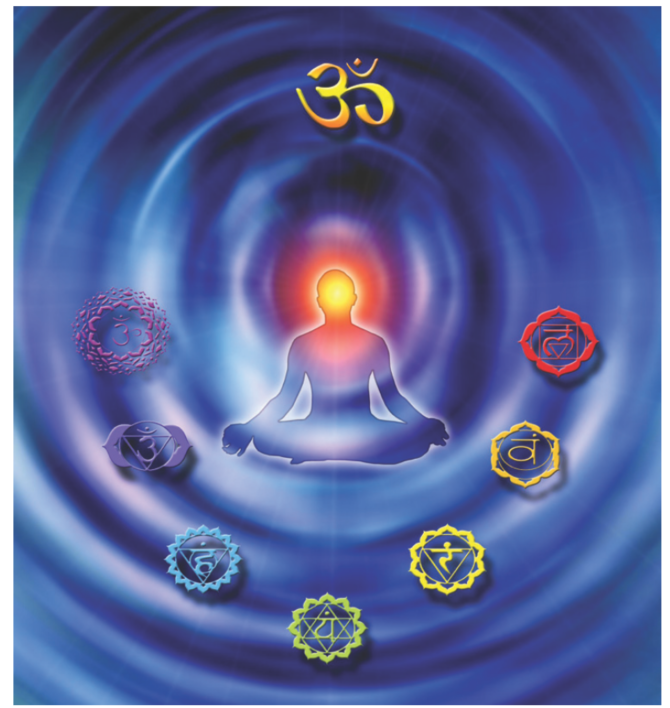
\includegraphics[width=\linewidth,keepaspectratio]{ycb1_pranav}

		{\tiny (Ref: Certification  of Yoga Professionals Official Guidebook For Level I (Instructor))}		
        \end{center}	
    \end{column}
\end{columns}
\end{frame}

%%%%%%%%%%%%%%%%%%%%%%%%%%%%%%%%%%%%%%%%%%%%%%%%%%%%%%%%%%%
\begin{frame}[fragile]\frametitle{Concept of Hymns}
\begin{columns}
    \begin{column}[T]{0.5\linewidth}
      \begin{itemize}
        \item \textbf{Hymns}: Sacred \textbf{verses} in Yoga.
        \item Integral to \textbf{rituals} and \textbf{devotional practices}.
        \item \textbf{Chanting} hymns invokes \textbf{spiritual energies}.
        \item \textbf{Vedic Hymns}: Ancient, transcendental \textbf{sound}.
        \item Used for \textbf{purification} and \textbf{blessings}.
      \end{itemize}
    \end{column}
    \begin{column}[T]{0.5\linewidth}
        \begin{center}
        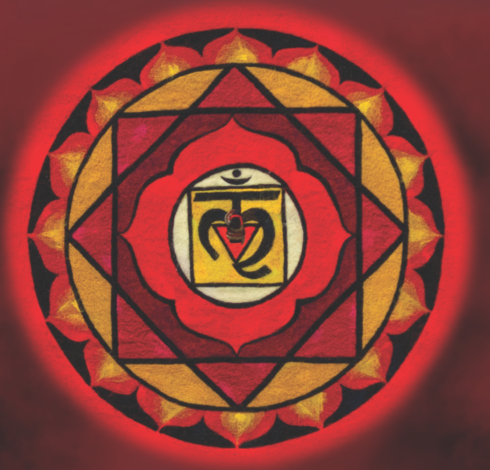
\includegraphics[width=\linewidth,keepaspectratio]{ycb1_hymns}

		{\tiny (Ref: Certification  of Yoga Professionals Official Guidebook For Level I (Instructor))}	
        \end{center}	
    \end{column}
\end{columns}
\end{frame}

% %%%%%%%%%%%%%%%%%%%%%%%%%%%%%%%%%%%%%%%%%%%%%%%%%%%%%%%%%%%
% \begin{frame}[fragile]\frametitle{Recitation of Hymns}
% \begin{columns}
    % \begin{column}[T]{0.5\linewidth}
      % \begin{itemize}
        % \item \textbf{Sanskrit Hymns}: Pronunciation and \textbf{intonation}.
        % \item Enhances \textbf{mental clarity} and \textbf{focus}.
        % \item \textbf{Spiritual growth} through regular recitation.
        % \item Commonly chanted during \textbf{Puja} and \textbf{Satsang}.
        % \item \textbf{Harmonizes} mind and spirit.
      % \end{itemize}
    % \end{column}
    % \begin{column}[T]{0.5\linewidth}
        % \begin{center}
        % 
\includegraphics[width=\linewidth,keepaspectratio]{ycb1_recite}

		% {\tiny (Ref: Certification  of Yoga Professionals Official Guidebook For Level I (Instructor))}	
        % \end{center}	
    % \end{column}
% \end{columns}
% \end{frame}


%%%%%%%%%%%%%%%%%%%%%%%%%%%%%%%%%%%%%%%%%%%%%%%%%%%%%%%%%%%%%%%%%%%%%%%%%%%%%%%%%%
\begin{frame}[fragile]\frametitle{}
\begin{center}
{\Large Yoga Cleansing Techniques}
\end{center}
\end{frame}

%%%%%%%%%%%%%%%%%%%%%%%%%%%%%%%%%%%%%%%%%%%%%%%%%%%%%%%%%%%
\begin{frame}[fragile]\frametitle{Dhauti}
\begin{columns}
    \begin{column}[T]{0.5\linewidth}
      \begin{itemize}
        \item \textbf{Dhauti} (\textit{धौती}): Cleansing of the \textbf{digestive tract}.
        \item Involves \textbf{internal purification}.
        \item Helps in removing \textbf{toxins} from the body.
        \item Types include \textbf{Vastra Dhauti} (\textit{वस्त्र धौती}) (cloth cleansing).
        \item Promotes \textbf{digestive health} and \textbf{detoxification}.
		\begin{itemize}
		  \item \textbf{Vaman Dhauti} (\textit{वमन धौती}): uses saline, tepid water.
		  \item \textbf{Danda Dhauti} (\textit{दण्ड धौती}): uses a rubber tube.
		  \item \textbf{Vastra Dhauti} (\textit{वस्त्र धौती}): uses a cloth strip.
		\end{itemize}		
      \end{itemize}
    \end{column}
    \begin{column}[T]{0.5\linewidth}
        \begin{center}
        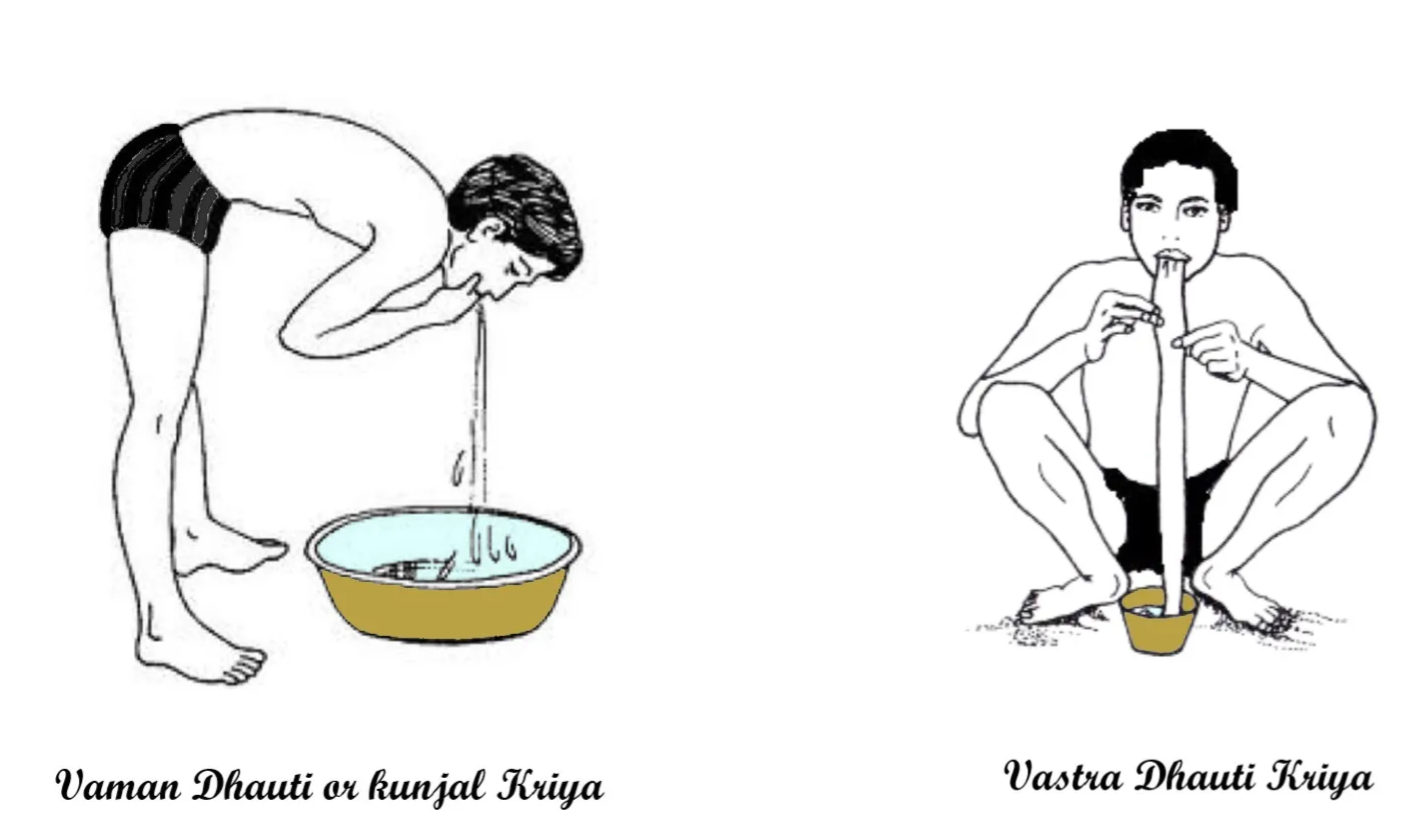
\includegraphics[width=\linewidth,keepaspectratio]{ycb1_dhauti}
		
		{\tiny (Ref: What is Shatkarma? 6 Types of Shatkarma for Purification and Their Benefits - Yogi Anurag)}	
        \end{center}	
    \end{column}
\end{columns}
\end{frame}


%%%%%%%%%%%%%%%%%%%%%%%%%%%%%%%%%%%%%%%%%%%%%%%%%%%%%%%%%%%
\begin{frame}[fragile]\frametitle{Neti}
\begin{columns}
    \begin{column}[T]{0.5\linewidth}
      \begin{itemize}
          \item \textbf{Neti} (\textit{नेति}) Kriya cleanses the nasal passages using a neti pot with salt lukewarm water.
          \item Two types of Neti:
            \begin{itemize}
              \item \textbf{Jala Neti} (\textit{जल नेति}): Uses water to cleanse nostrils by pouring water through one nostril and expelling it out the other.
              \item \textbf{Sutra Neti} (\textit{सूत्र नेति}): Uses a rubber thread to massage nasal pathways and open blockages.
            \end{itemize}
      \end{itemize}
    \end{column}
    \begin{column}[T]{0.5\linewidth}
        \begin{center}
        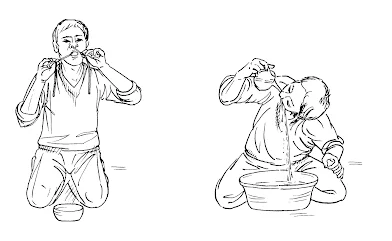
\includegraphics[width=\linewidth,keepaspectratio]{ycb1_neti}
		
		{\tiny (Ref: What is Shatkarma? 6 Types of Shatkarma for Purification and Their Benefits - Yogi Anurag)}	
        \end{center}	
    \end{column}
\end{columns}
\end{frame}


%%%%%%%%%%%%%%%%%%%%%%%%%%%%%%%%%%%%%%%%%%%%%%%%%%%%%%%%%%%
\begin{frame}[fragile]\frametitle{Kapalabhati}
\begin{columns}
    \begin{column}[T]{0.5\linewidth}
      \begin{itemize}
          \item \textbf{Kapalabhati} (\textit{कपालभाती}) cleanses the frontal lobes and improves brain function.
          \item Known as Kapalabhati pranayama (\textit{कपालभाती प्राणायाम}), it is a breathing technique.
          \item Involves rapid movement of the abdominal wall with breathing.
          \item In normal breathing, inhalation is active and exhalation is passive.
          \item In Kapalabhati breathing, exhalation is active and inhalation is passive.
          \item Emphasizing exhalation helps expel more impurities as CO2.
      \end{itemize}
    \end{column}
    \begin{column}[T]{0.5\linewidth}
        \begin{center}
        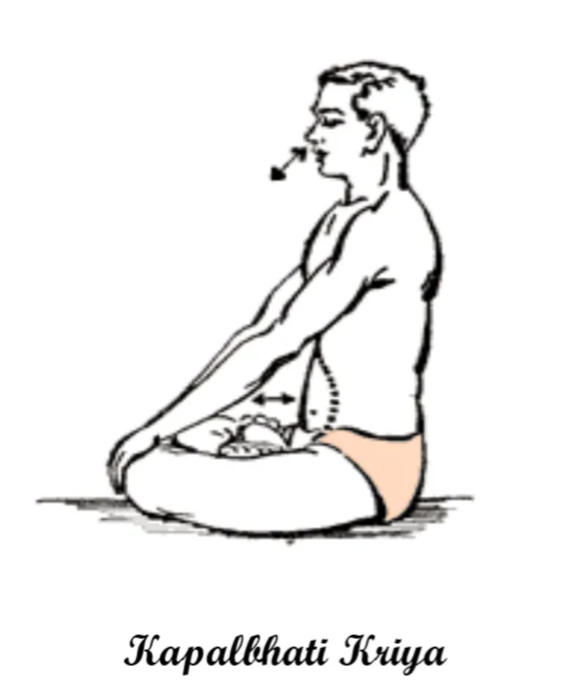
\includegraphics[width=0.8\linewidth,keepaspectratio]{ycb1_kapalbhati}
		
		{\tiny (Ref: What is Shatkarma? 6 Types of Shatkarma for Purification and Their Benefits - Yogi Anurag)}	
        \end{center}	
    \end{column}
\end{columns}
\end{frame}


%%%%%%%%%%%%%%%%%%%%%%%%%%%%%%%%%%%%%%%%%%%%%%%%%%%%%%%%%%%
\begin{frame}[fragile]\frametitle{Nauli}
\begin{columns}
    \begin{column}[T]{0.6\linewidth}
      \begin{itemize}
          \item \textbf{Nauli} (\textit{नौली}) Kriya cleanses abdominal organs through massaging.
          \item Purifies liver, spleen, urinary bladder, pancreas, gall bladder, and intestines.
          \item Regular practice improves digestion and appetite.
          \item Involves isolating \textbf{rectus abdominis} (\textit{अन्तरत्वक}) muscles.
          \item Abs muscles can be isolated left, right, or middle of the linea alba (\textit{लिनिया अल्बा}).
          \item Three types of Nauli:
            \begin{itemize}
              \item \textbf{Madhya Nauli} (\textit{मध्य नौली}): Abs muscles concentrated at the center (linea alba).
              \item \textbf{Vama Nauli} (\textit{वाम नौली}): Abs muscles aligned to the left of the center.
              \item \textbf{Dakshina Nauli} (\textit{दक्षिण नौली}): Abs muscles aligned to the right of the center.
            \end{itemize}
      \end{itemize}
    \end{column}
    \begin{column}[T]{0.4\linewidth}
        \begin{center}
        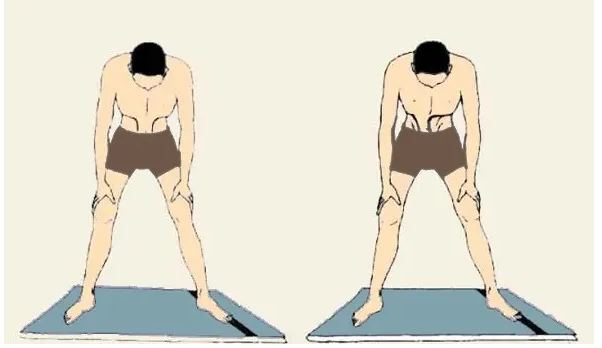
\includegraphics[width=\linewidth,keepaspectratio]{ycb1_nauli}
		
		{\tiny (Ref: What is Shatkarma? 6 Types of Shatkarma for Purification and Their Benefits - Yogi Anurag)}	
        \end{center}	
    \end{column}
\end{columns}	  
\end{frame}


%%%%%%%%%%%%%%%%%%%%%%%%%%%%%%%%%%%%%%%%%%%%%%%%%%%%%%%%%%%
\begin{frame}[fragile]\frametitle{Trataka}
\begin{columns}
    \begin{column}[T]{0.5\linewidth}
     \begin{itemize}
          \item \textbf{Trataka} (\textit{त्राटक}) Kriya cleanses and exercises the eyes.
          \item Involves steady and continuous gazing at a reference point.
          \item Common reference point: Illuminated candle.
          \item Consistent practice increases concentration power.
          \item Two types of Trataka:
            \begin{itemize}
              \item \textbf{Internal Trataka} (\textit{आन्तरिक त्राटक}): Focus on \textbf{trikuti} (\textit{त्रिकुटी}) (third eye) between eyebrows.
              \item \textbf{External Trataka} (\textit{बाह्य त्राटक}): Gazing at external objects that provide pleasure.
            \end{itemize}
      \end{itemize}
    \end{column}
    \begin{column}[T]{0.5\linewidth}
        \begin{center}
        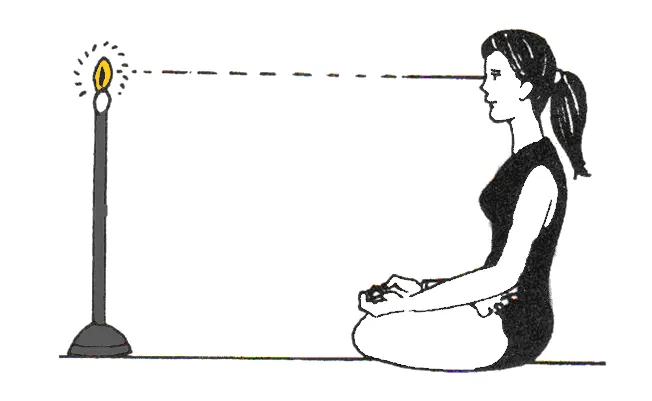
\includegraphics[width=\linewidth,keepaspectratio]{ycb1_tratak}
		
		{\tiny (Ref: What is Shatkarma? 6 Types of Shatkarma for Purification and Their Benefits - Yogi Anurag)}	
        \end{center}	
    \end{column}
\end{columns}	  
\end{frame}

%%%%%%%%%%%%%%%%%%%%%%%%%%%%%%%%%%%%%%%%%%%%%%%%%%%%%%%%%%%
\begin{frame}[fragile]\frametitle{Basti}
\begin{columns}
    \begin{column}[T]{0.5\linewidth}
      \begin{itemize}
          \item \textbf{Basti} (\textit{बस्ती}) Kriya cleanses the large intestine and cures 50\% of abdominal diseases.
          \item Two types of Basti:
            \begin{itemize}
              \item \textbf{Sthala Basti} (\textit{स्थल बस्ती})
              \item \textbf{Jala Basti} (\textit{जल बस्ती})
            \end{itemize}
          \item In both techniques, water is drawn in through the anus into the large intestine.
          \item Abdominal muscles are churned while holding water inside.
          \item Water is then expelled out through the anus.
          \item Purifies the colon, which nourishes almost all tissues of the body.
      \end{itemize}
    \end{column}
    \begin{column}[T]{0.5\linewidth}
        \begin{center}
        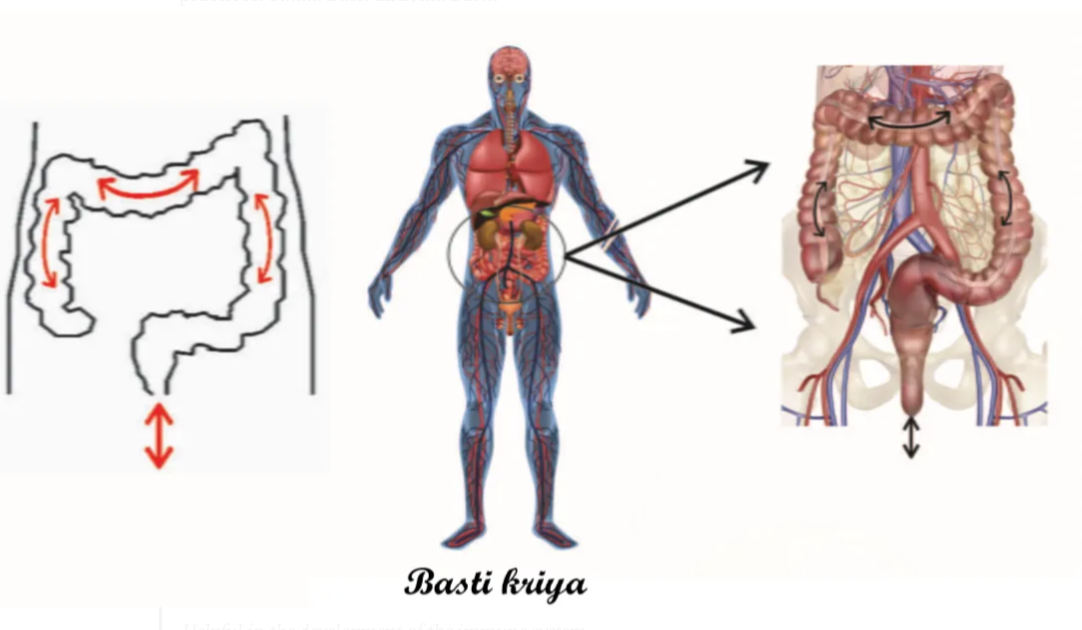
\includegraphics[width=\linewidth,keepaspectratio]{ycb1_basti}
		
		{\tiny (Ref: What is Shatkarma? 6 Types of Shatkarma for Purification and Their Benefits - Yogi Anurag)}	
        \end{center}	
    \end{column}
\end{columns}	  
\end{frame}


%%%%%%%%%%%%%%%%%%%%%%%%%%%%%%%%%%%%%%%%%%%%%%%%%%%%%%%%%%%%%%%%%%%%%%%%%%%%%%%%%%
\begin{frame}[fragile]\frametitle{}
\begin{center}
{\Large योगिक सूक्ष्म व्यायाम  Yogic Sukshma Vyayama and स्थूल व्यायाम Sthula Vyayama}
\end{center}
\end{frame}


%%%%%%%%%%%%%%%%%%%%%%%%%%%%%%%%%%%%%%%%%%%%%%%%%%%%%%%%%%%
\begin{frame}[fragile]\frametitle{Sukshma Vyayama: Concept}
\begin{columns}
    \begin{column}[T]{0.5\linewidth}
      \begin{itemize}
        \item \textbf{Sukshma Vyayama}: Subtle \textbf{exercise} in Yoga.
        \item Focuses on \textbf{micro-movements} and \textbf{joints}.
        \item Enhances \textbf{flexibility} and \textbf{joint mobility}.
        \item Aims to \textbf{prepare the body} for more intense practices.
        \item Often used as a \textbf{warm-up} in Yoga sessions.
		  \begin{itemize}
			\item \textbf{Neck rotations}: Improves \textbf{neck flexibility}.
			\item \textbf{Shoulder rolls}: Enhances \textbf{shoulder mobility}.
			\item \textbf{Wrist and ankle movements}: Prepares \textbf{joints}.
			\item \textbf{Spinal twists}: Facilitates \textbf{spinal flexibility}.
			\item \textbf{Toe touches}: Stretches \textbf{hamstrings}.
		  \end{itemize}		
      \end{itemize}
    \end{column}
    \begin{column}[T]{0.5\linewidth}
        \begin{center}
			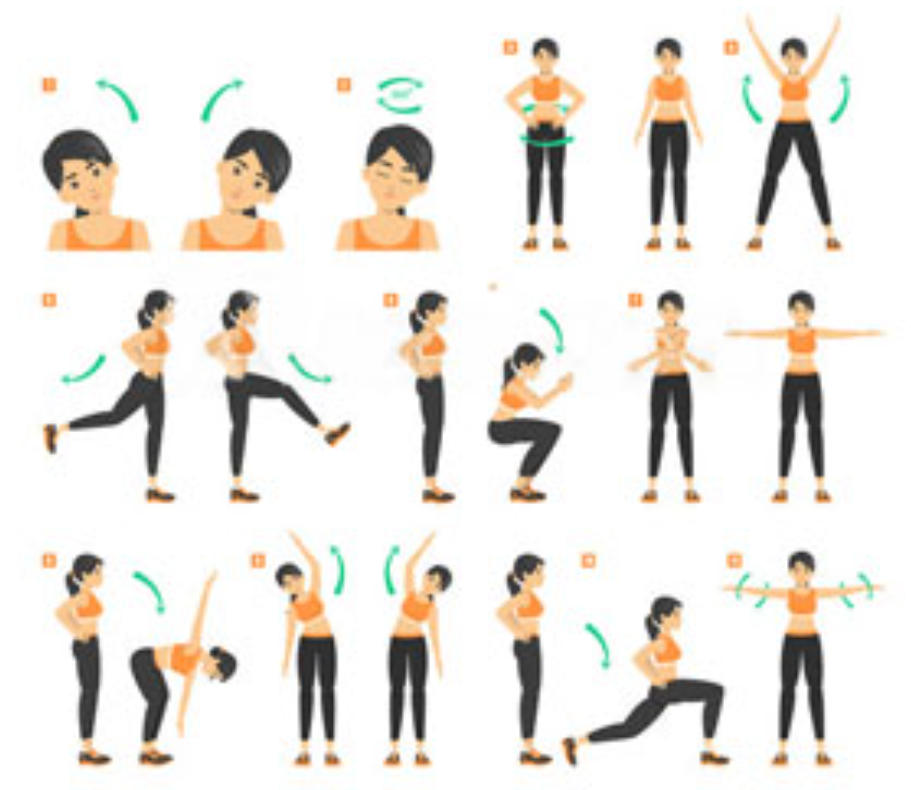
\includegraphics[width=\linewidth,keepaspectratio]{ycb1_sukshma}
				
			{\tiny (Ref: Sukshma vyayama: The 7-minute relaxation exercise Activating the Joints)}		
        \end{center}	
    \end{column}
\end{columns}
\end{frame}

%%%%%%%%%%%%%%%%%%%%%%%%%%%%%%%%%%%%%%%%%%%%%%%%%%%%%%%%%%%
\begin{frame}[fragile]\frametitle{Neck Movement}
\begin{columns}
    \begin{column}[T]{0.5\linewidth}
      \begin{itemize}
		\item \textbf{Griva Shakti Vikasaka I (ग्रीवा शक्ति विकासक I)}: Forward and backward bending
		\item \textbf{Griva Shakti Vikasaka II (ग्रीवा शक्ति विकासक II)}: Right and Left bending
		\item \textbf{Griva Shakti Vikasaka III (ग्रीवा शक्ति विकासक III)}: Right and Left Twisting
		\item \textbf{Griva Shakti Vikasaka IV (ग्रीवा शक्ति विकासक IV)}: Neck Rotation
		\item \textbf{Benefits (लाभ)}: Enhances flexibility and strength
	  \end{itemize}
	  
				{\tiny (Ref: Day 02 of 30 Days of Yogic Journey — Guiding Principles for Yoga Practitioners and Yogic Sukshma Vyayama - Saatvik Life)}		  
    \end{column}
    \begin{column}[T]{0.5\linewidth}
		\begin{center}
		I, III, IV
		
		        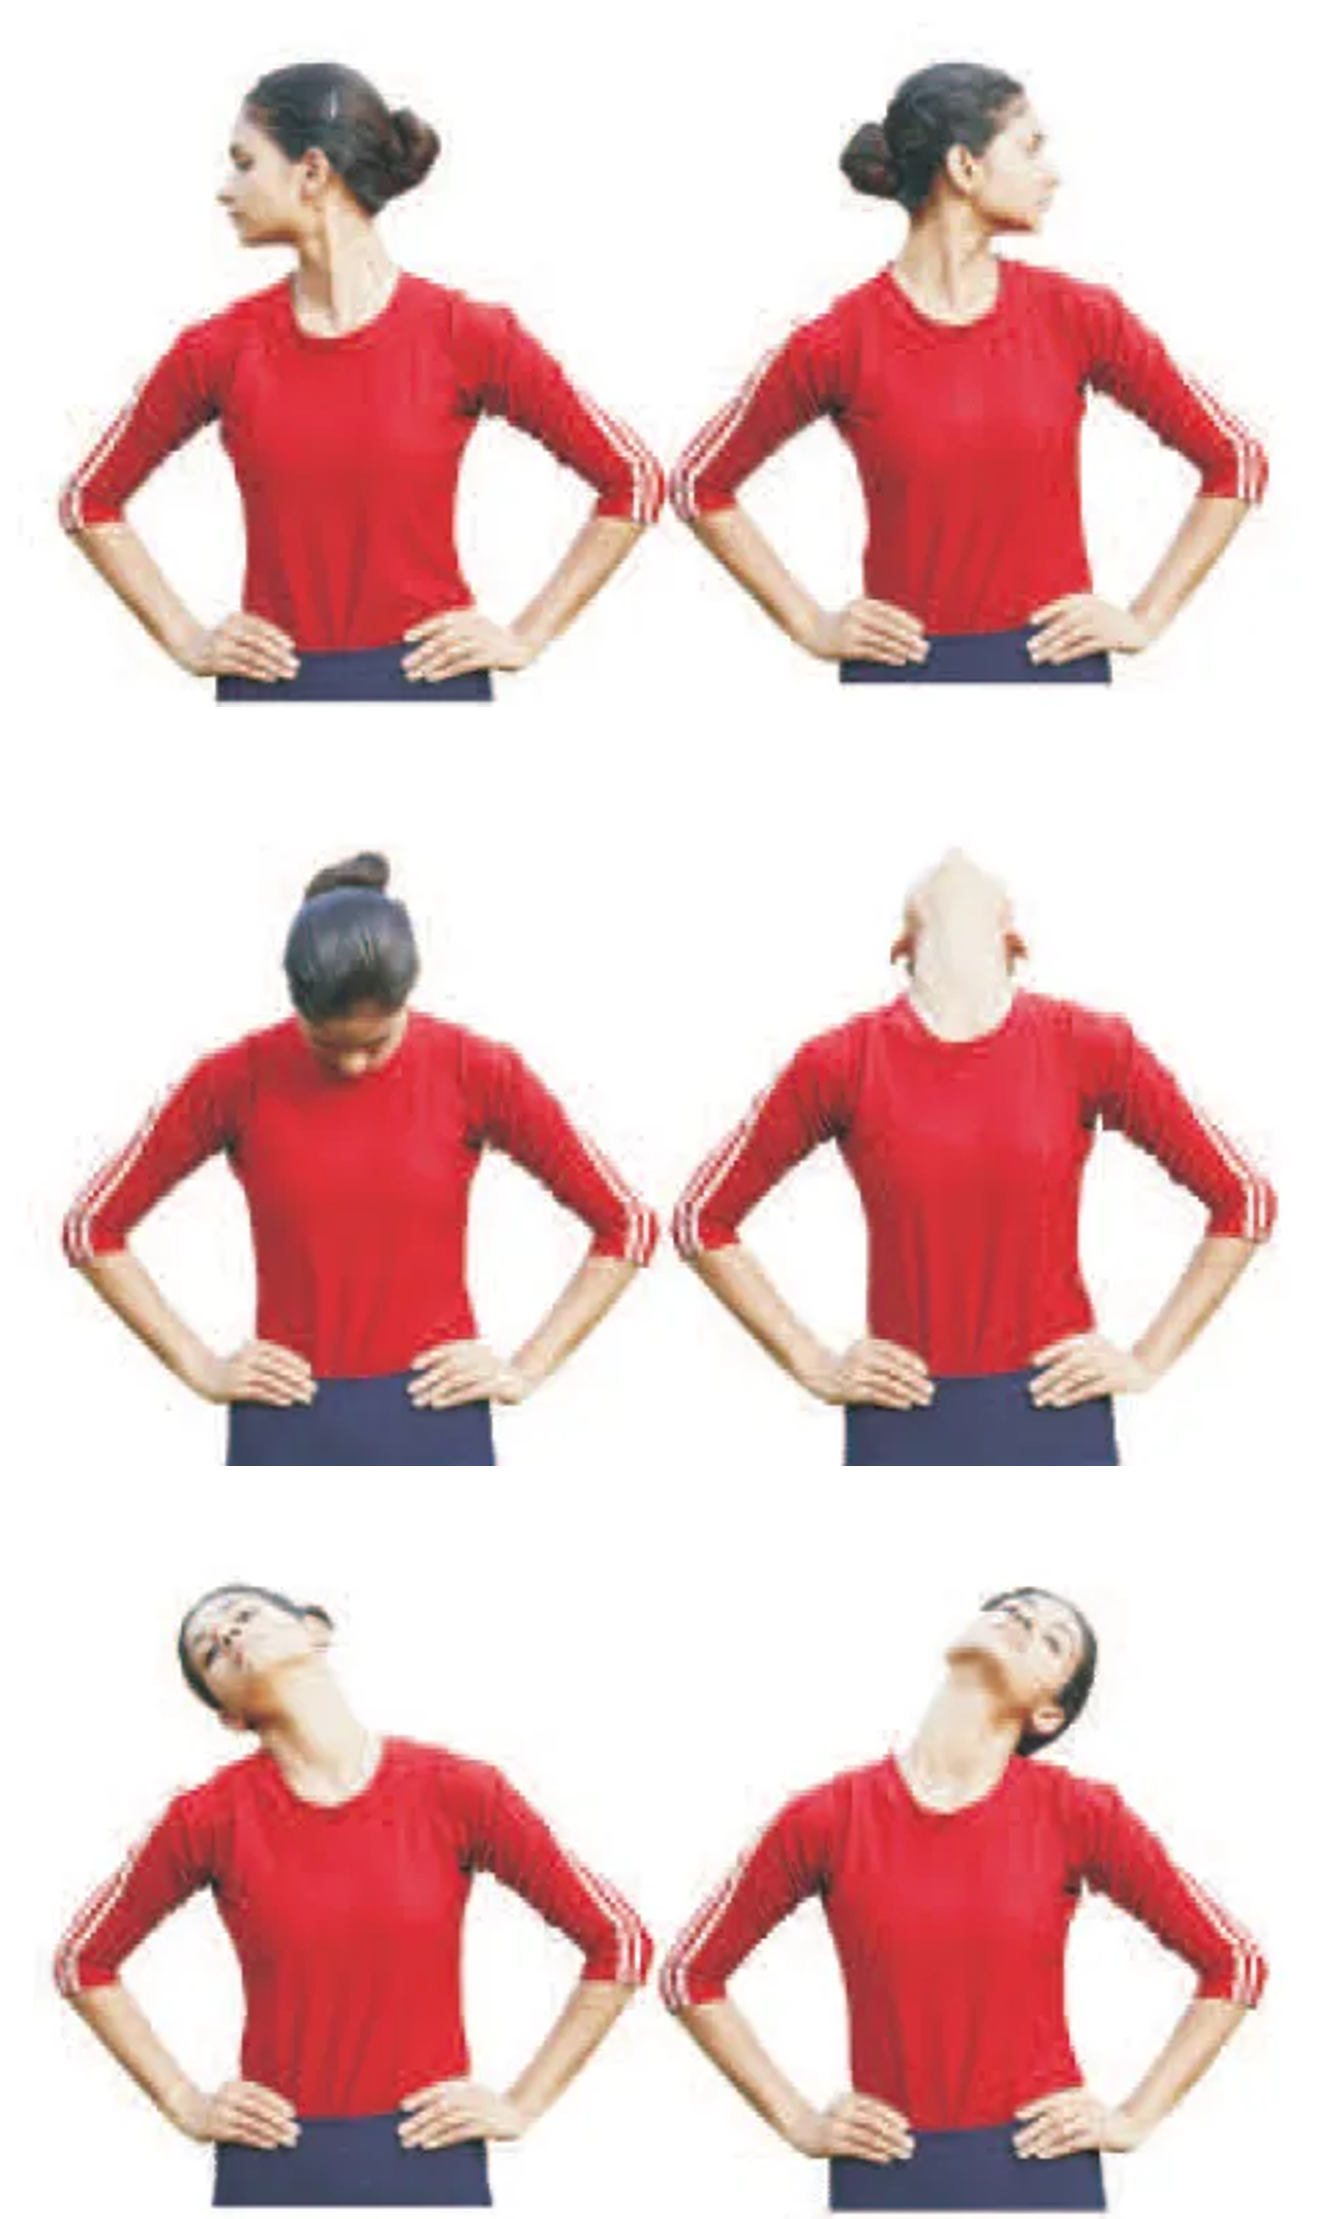
\includegraphics[width=0.5\linewidth,keepaspectratio]{ycb1_greeva}
				
				
		II
		
				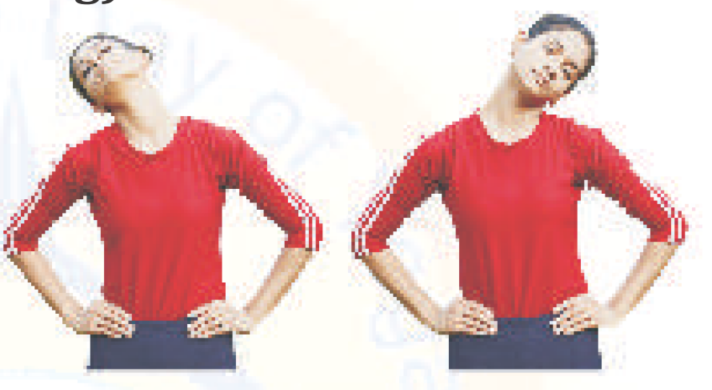
\includegraphics[width=0.5\linewidth,keepaspectratio]{ycb1_greevabend}

	
		\end{center}	
    \end{column}
\end{columns}

\end{frame}


%%%%%%%%%%%%%%%%%%%%%%%%%%%%%%%%%%%%%%%%%%%%%%%%%%%%%%%%%%%
\begin{frame}[fragile]\frametitle{Shoulder Movement}
\begin{columns}
    \begin{column}[T]{0.5\linewidth}
      \begin{itemize}
		\item \textbf{Bhuja Valli Shakti Vikasaka (भुजा वल्ली शक्ति विकासक)}: Arm circles
		\item \textbf{Bhuja Valli Shakti Vikasaka (भुजा वल्ली शक्ति विकासक)}: Shoulder shrugs
		\item \textbf{Purna Bhuja Shakti Vikasaka (पूर्ण भुजा शक्ति विकासक)}: Shoulder rotations
		\item \textbf{Purna Bhuja Shakti Vikasaka (पूर्ण भुजा शक्ति विकासक)}: Arm raises
		\item \textbf{Benefits (लाभ)}: Increases range of motion and strength
	  \end{itemize}
    \end{column}
    \begin{column}[T]{0.5\linewidth}
		\begin{center}
		        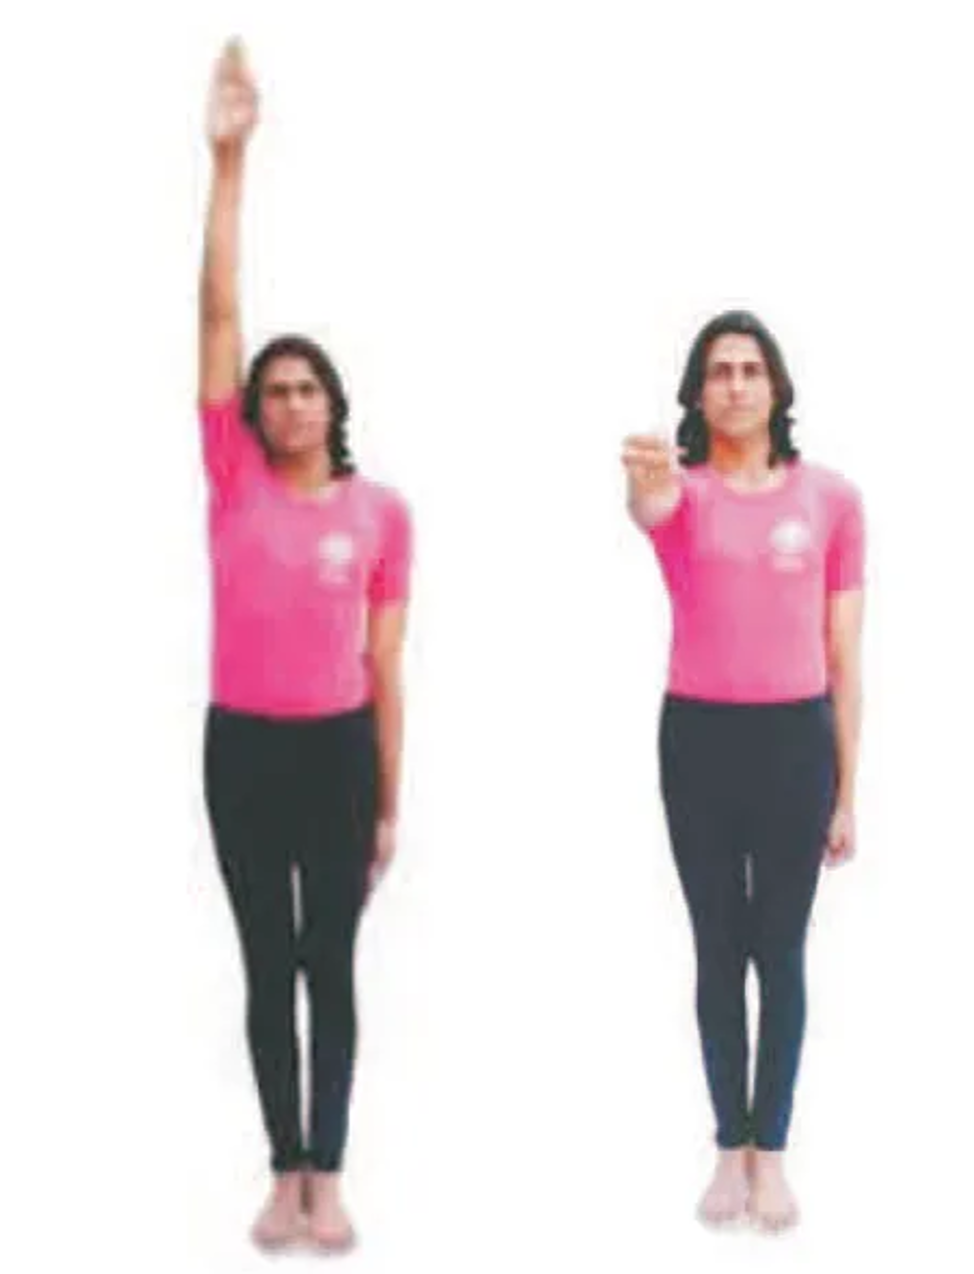
\includegraphics[width=0.7\linewidth,keepaspectratio]{ycb1_bhuja}
				
				{\tiny (Ref: Day 02 of 30 Days of Yogic Journey — Guiding Principles for Yoga Practitioners and Yogic Sukshma Vyayama - Saatvik Life)}		
		\end{center}	
    \end{column}
\end{columns}
\end{frame}


%%%%%%%%%%%%%%%%%%%%%%%%%%%%%%%%%%%%%%%%%%%%%%%%%%%%%%%%%%%
\begin{frame}[fragile]\frametitle{Trunk Movement}
\begin{columns}
    \begin{column}[T]{0.5\linewidth}
      \begin{itemize}
		\item \textbf{Kati Shakti Vikasaka I (कटी शक्ति विकासक I)}: Side bends
		\item \textbf{Kati Shakti Vikasaka II (कटी शक्ति विकासक II)}: Forward bends
		\item \textbf{Kati Shakti Vikasaka III (कटी शक्ति विकासक III)}: Backward bends
		\item \textbf{Kati Shakti Vikasaka IV (कटी शक्ति विकासक IV)}: Twists
		\item \textbf{Kati Shakti Vikasaka V (कटी शक्ति विकासक V)}: Rotational stretches
		\item \textbf{Benefits (लाभ)}: Strengthens core, improves flexibility
	  \end{itemize}
    \end{column}
    \begin{column}[T]{0.5\linewidth}
		\begin{center}
		        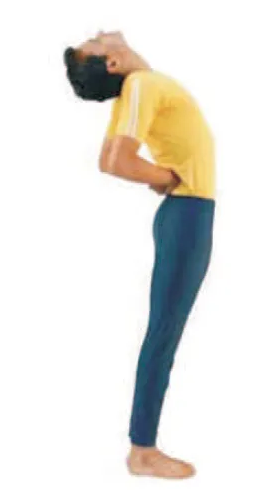
\includegraphics[width=0.5\linewidth,keepaspectratio]{ycb1_kati}
				
				{\tiny (Ref: Day 02 of 30 Days of Yogic Journey — Guiding Principles for Yoga Practitioners and Yogic Sukshma Vyayama - Saatvik Life)}	
		\end{center}	
    \end{column}
\end{columns}
\end{frame}

%%%%%%%%%%%%%%%%%%%%%%%%%%%%%%%%%%%%%%%%%%%%%%%%%%%%%%%%%%%
\begin{frame}[fragile]\frametitle{Knee Movement}
\begin{columns}
    \begin{column}[T]{0.5\linewidth}
      \begin{itemize}
		% \item \textbf{Jangha Shakti Vikasaka II-A (जंघ शक्ति विकासक II-A)}: Knee lifts
		% \item \textbf{Jangha Shakti Vikasaka II-B (जंघ शक्ति विकासक II-B)}: Knee bends
		\item \textbf{Janu Shakti Vikasaka (जनु शक्ति विकासक)}: Knee rotations
		\item \textbf{Janu Shakti Vikasaka (जनु शक्ति विकासक)}: Side stretches
		\item \textbf{Benefits (लाभ)}: Enhances knee strength and flexibility
	  \end{itemize}
	  
	  		{\tiny (Ref: Day 03 of 30 Days of Yogic Journey — Guiding Principles for Yoga Practitioners and Yogic Sukshma Vyayama - Saatvik Life)}	
    \end{column}
    \begin{column}[T]{0.5\linewidth}
		\begin{center}
		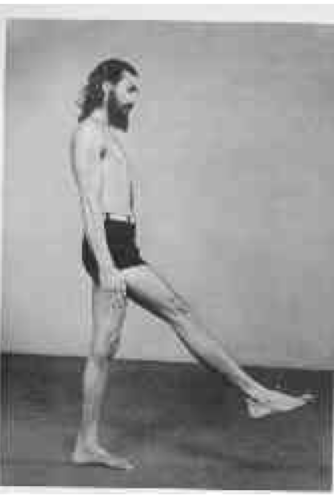
\includegraphics[width=0.4\linewidth,keepaspectratio]{ycb1_janu_1}
		
		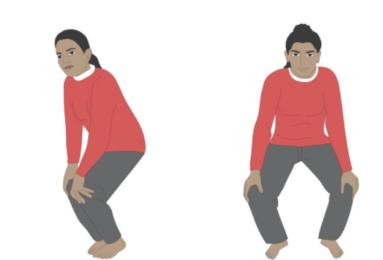
\includegraphics[width=0.4\linewidth,keepaspectratio]{ycb1_janu_2}

		\end{center}	
    \end{column}
\end{columns}
\end{frame}

%%%%%%%%%%%%%%%%%%%%%%%%%%%%%%%%%%%%%%%%%%%%%%%%%%%%%%%%%%%
\begin{frame}[fragile]\frametitle{Thighs Movement}
\begin{columns}
    \begin{column}[T]{0.5\linewidth}
      \begin{itemize}
		\item \textbf{Jangha Shakti Vikasaka II-A (जंघ शक्ति विकासक II-A)}: Jumping Jacks
		\item \textbf{Jangha Shakti Vikasaka II-B (जंघ शक्ति विकासक II-B)}: Thighs bends, sit with hands front
		% \item \textbf{Janu Shakti Vikasaka (जनु शक्ति विकासक)}: Knee rotations
		% \item \textbf{Janu Shakti Vikasaka (जनु शक्ति विकासक)}: Side stretches
		\item \textbf{Benefits (लाभ)}: Enhances thighs strength and flexibility
	  \end{itemize}
	  
		{\tiny (Ref: Day 03 of 30 Days of Yogic Journey — Guiding Principles for Yoga Practitioners and Yogic Sukshma Vyayama - Saatvik Life)}		  
    \end{column}
    \begin{column}[T]{0.5\linewidth}
		\begin{center}
		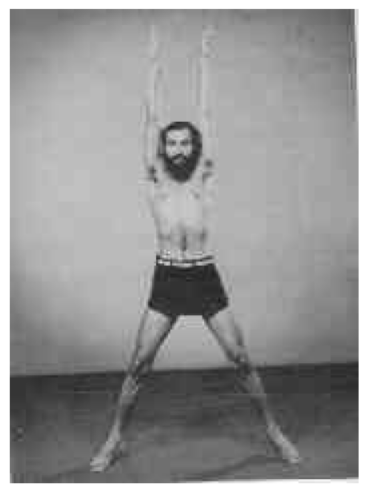
\includegraphics[width=0.5\linewidth,keepaspectratio]{ycb1_jangha_1}
		
		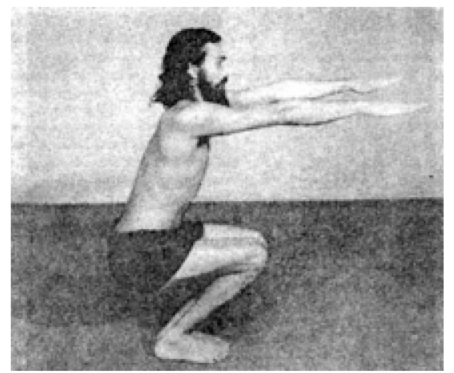
\includegraphics[width=0.5\linewidth,keepaspectratio]{ycb1_jangha_2}


		\end{center}	
    \end{column}
\end{columns}
\end{frame}


%%%%%%%%%%%%%%%%%%%%%%%%%%%%%%%%%%%%%%%%%%%%%%%%%%%%%%%%%%%
\begin{frame}[fragile]\frametitle{Ankle Movement}
 \begin{columns}
    \begin{column}[T]{0.5\linewidth}
      \begin{itemize}
		\item \textbf{Pada-mula Shakti Vikasaka A (पाद-मूल शक्ति विकासक A)}: Ankle circles
		\item \textbf{Pada-mula Shakti Vikasaka B (पाद-मूल शक्ति विकासक B)}: Flexion and extension
		\item \textbf{Gulpha-pada-pristha-pada-tala Shakti Vikasaka (गुल्फ-पाद-पृष्ठ-पाद-तल शक्ति विकासक)}: Foot stretches
		\item \textbf{Gulpha-pada-pristha-pada-tala Shakti Vikasaka (गुल्फ-पाद-पृष्ठ-पाद-तल शक्ति विकासक)}: Heel raises
		\item \textbf{Benefits (लाभ)}: Improves ankle mobility and strength
	  \end{itemize}
    \end{column}
    \begin{column}[T]{0.5\linewidth}
		\begin{center}
		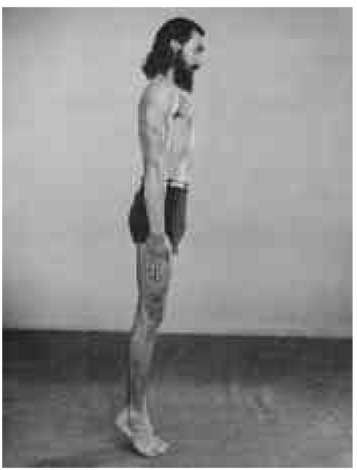
\includegraphics[width=0.5\linewidth,keepaspectratio]{ycb1_pada}
		
		
		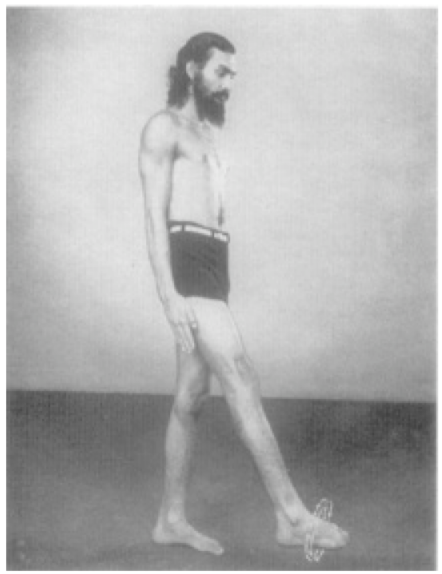
\includegraphics[width=0.5\linewidth,keepaspectratio]{ycb1_gulpha}
		
		\end{center}	
    \end{column}
\end{columns}
\end{frame}


%%%%%%%%%%%%%%%%%%%%%%%%%%%%%%%%%%%%%%%%%%%%%%%%%%%%%%%%%%%
\begin{frame}[fragile]\frametitle{Sthula Vyayama: Concept}
\begin{columns}
    \begin{column}[T]{0.5\linewidth}
      \begin{itemize}
        \item \textbf{Sthula Vyayama}: Gross \textbf{exercise} in Yoga.
        \item Focuses on \textbf{muscle strength} and \textbf{physical endurance}.
        \item Includes \textbf{dynamic movements} and \textbf{stretches}.
        \item Aims to \textbf{build strength} and \textbf{stamina}.
        \item Often part of \textbf{physical Yoga routines}.
			  \begin{itemize}
				\item \textbf{Push-ups}: Strengthens \textbf{upper body}.
				\item \textbf{Squats}: Builds \textbf{leg muscles}.
				\item \textbf{Planks}: Engages \textbf{core muscles}.
				\item \textbf{Lunges}: Improves \textbf{lower body strength}.
				\item \textbf{Leg raises}: Strengthens \textbf{abdominal muscles}.
			  \end{itemize}		
      \end{itemize}
    \end{column}
    \begin{column}[T]{0.5\linewidth}
        \begin{center}
		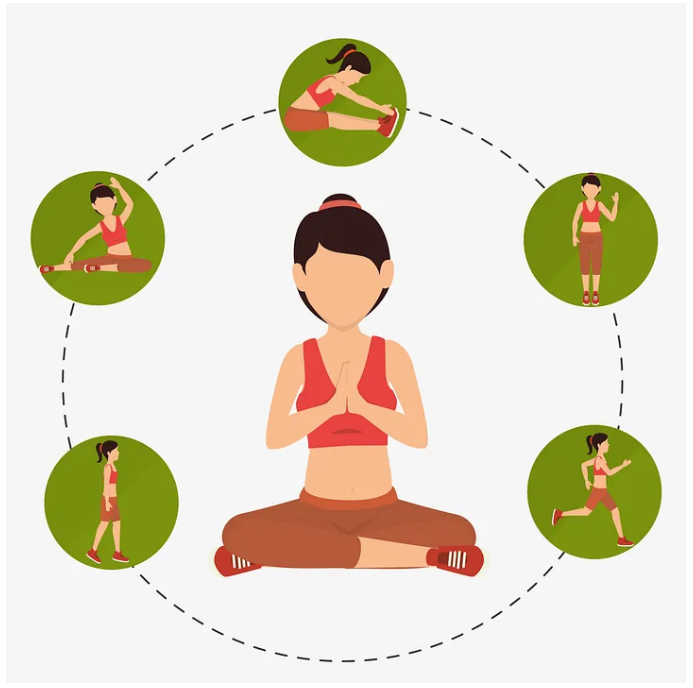
\includegraphics[width=\linewidth,keepaspectratio]{ycb1_sthula}
		
		{\tiny (Ref: Day 06 of 30 Days of Yogic Journey — Guiding Principles for Yoga Practitioners and Yogic Sukshma Vyayama - Saatvik Life)}	
        \end{center}	
    \end{column}
\end{columns}
\end{frame}

% %%%%%%%%%%%%%%%%%%%%%%%%%%%%%%%%%%%%%%%%%%%%%%%%%%%%%%%%%%%
% \begin{frame}[fragile]\frametitle{Examples of Sthula Vyayama}
% \begin{columns}
    % \begin{column}[T]{0.5\linewidth}
      % \begin{itemize}
        % \item \textbf{Push-ups}: Strengthens \textbf{upper body}.
        % \item \textbf{Squats}: Builds \textbf{leg muscles}.
        % \item \textbf{Planks}: Engages \textbf{core muscles}.
        % \item \textbf{Lunges}: Improves \textbf{lower body strength}.
        % \item \textbf{Leg raises}: Strengthens \textbf{abdominal muscles}.
      % \end{itemize}
    % \end{column}
    % \begin{column}[T]{0.5\linewidth}
        % \begin{center}
        % \includegraphics[width=\linewidth,keepaspectratio]{logo_yhk}
        % \end{center}	
    % \end{column}
% \end{columns}
% \end{frame}

%%%%%%%%%%%%%%%%%%%%%%%%%%%%%%%%%%%%%%%%%%%%%%%%%%%%%%%%%%%
\begin{frame}[fragile]\frametitle{Sarvanga Pushti}
\begin{columns}
    \begin{column}[T]{0.5\linewidth}
      \begin{itemize}
		\item \textbf{Sarvanga Pushti}: Full-body strength exercise
		\item \textbf{Objective}: Enhance overall muscular strength
		\item \textbf{Execution}: Perform with controlled movements
		\item \textbf{Focus}: Engage all major muscle groups
		\item \textbf{Benefits}: Improves strength, endurance, and balance
	  \end{itemize}
    \end{column}
    \begin{column}[T]{0.5\linewidth}
		\begin{center}
		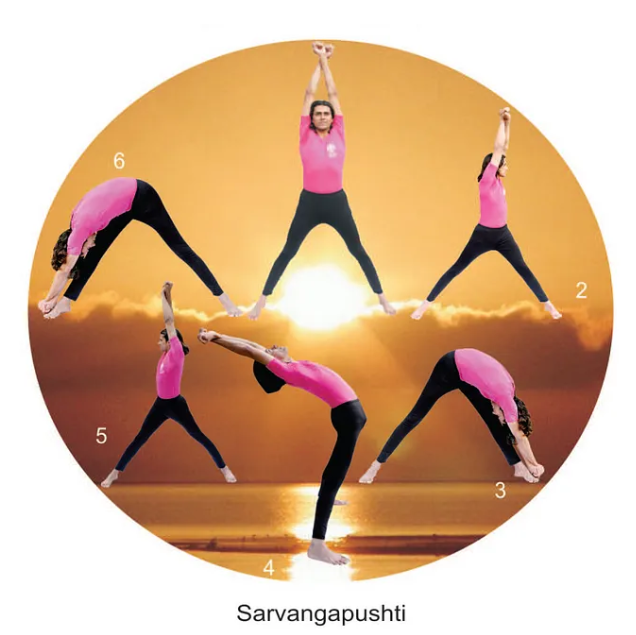
\includegraphics[width=\linewidth,keepaspectratio]{ycb1_sthula_sarvanga}
		
		{\tiny (Ref: Day 04 of 30 Days of Yogic Journey — Guiding Principles for Yoga Practitioners and Yogic Sukshma Vyayama - Saatvik Life)}	
		\end{center}	
    \end{column}
\end{columns}
\end{frame}

%%%%%%%%%%%%%%%%%%%%%%%%%%%%%%%%%%%%%%%%%%%%%%%%%%%%%%%%%%%
\begin{frame}[fragile]\frametitle{Hrid Gati (Engine Daud)}
\begin{columns}
    \begin{column}[T]{0.5\linewidth}
      \begin{itemize}
		\item \textbf{Hrid Gati}: Cardio exercise mimicking running
		\item \textbf{Objective}: Improve cardiovascular health
		\item \textbf{Execution}: Perform in a rhythmic, steady pace
		\item \textbf{Focus}: Maintain consistent breathing and pace
		\item \textbf{Benefits}: Boosts heart health, endurance, and stamina
	  \end{itemize}
    \end{column}
    \begin{column}[T]{0.5\linewidth}
		\begin{center}
		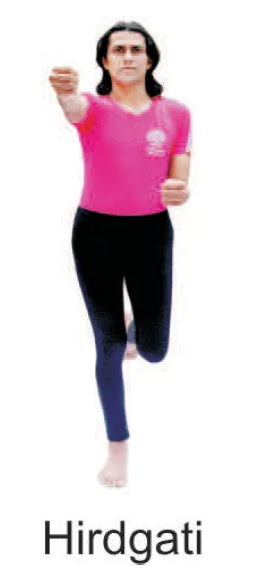
\includegraphics[width=0.5\linewidth,keepaspectratio]{ycb1_sthula_hrid}
		
		{\tiny (Ref: Day 04 of 30 Days of Yogic Journey — Guiding Principles for Yoga Practitioners and Yogic Sukshma Vyayama - Saatvik Life)}	
		\end{center}	
    \end{column}
\end{columns}
\end{frame}

%%%%%%%%%%%%%%%%%%%%%%%%%%%%%%%%%%%%%%%%%%%%%%%%%%%%%%%%%%%
\begin{frame}[fragile]\frametitle{Comparison of Sukshma and Sthula Vyayama}

      \begin{itemize}
        \item \textbf{Sukshma Vyayama}: Focus on \textbf{joints} and \textbf{flexibility}.
        \item \textbf{Sthula Vyayama}: Targets \textbf{muscle strength} and \textbf{endurance}.
        \item \textbf{Sukshma}: \textbf{Gentle} and \textbf{subtle movements}.
        \item \textbf{Sthula}: \textbf{Dynamic} and \textbf{strength-based exercises}.
        \item Both \textbf{complement each other} in a balanced Yoga practice.
      \end{itemize}

\end{frame}


%%%%%%%%%%%%%%%%%%%%%%%%%%%%%%%%%%%%%%%%%%%%%%%%%%%%%%%%%%%%%%%%%%%%%%%%%%%%%%%%%%
\begin{frame}[fragile]\frametitle{}
\begin{center}
{\Large Yogic Surya Namaskara}
\end{center}
\end{frame}

%%%%%%%%%%%%%%%%%%%%%%%%%%%%%%%%%%%%%%%%%%%%%%%%%%%%%%%%%%%
\begin{frame}[fragile]\frametitle{Surya Namaskara: Concept}
      \begin{itemize}
        \item \textbf{Surya Namaskara}: Sun \textbf{Salutation}.
        \item Integral part of \textbf{Hatha Yoga}.
        \item Consists of a sequence of \textbf{12 postures}.
        \item Aims to \textbf{energize} and \textbf{purify} the body.
        \item Traditionally performed \textbf{facing the sunrise}.
		\item Benefits of Surya Namaskara
		      \begin{itemize}
			\item Improves \textbf{flexibility} and \textbf{strength}.
			\item Enhances \textbf{circulation} and \textbf{digestion}.
			\item Promotes \textbf{mental calmness} and \textbf{focus}.
			\item Helps in \textbf{weight management} and \textbf{detoxification}.
			\item Strengthens the \textbf{immune system}.
		\item Precaution and Tips
		  \begin{itemize}
			\item Perform on an \textbf{empty stomach}.
			\item Avoid if you have \textbf{back pain} or \textbf{injuries}.
			\item Practice in a \textbf{well-ventilated} area.
			\item Keep the \textbf{breathing smooth} and \textbf{steady}.
			\item Focus on \textbf{alignment} and \textbf{posture}.
		  \end{itemize}		
		  \end{itemize}
      \end{itemize}

\end{frame}

%%%%%%%%%%%%%%%%%%%%%%%%%%%%%%%%%%%%%%%%%%%%%%%%%%%%%%%%%%%
\begin{frame}[fragile]\frametitle{Sequence of Surya Namaskara}

      \begin{itemize}
        \item \textbf{1. Pranamasana (प्रणामासना)}: Prayer Pose.
        \item \textbf{2. Hasta Uttanasana (हस्त उत्तानासन)}: Raised Arms Pose.
        \item \textbf{3. Padahastasana (पदहस्तासन)}: Hand to Foot Pose.
        \item \textbf{4. Ashwa Sanchalanasana (अश्व संचारणासन)}: Equestrian Pose.
        \item \textbf{5. Chanturang Dandasana (चतुरंग दंडासन)}: Plank Pose.
        \item \textbf{6. Ashtanga Namaskara (अष्टांग नमस्कार)}: Salute with Eight Points.
        \item \textbf{7. Bhujangasana (भुजंगासन)}: Cobra Pose.
        \item \textbf{8. Adho Mukha Svanasana (अधोमुख श्वानासन)}: Downward Facing Dog.
        \item \textbf{9. Ashwa Sanchalanasana (अश्व संचारणासन)}: Equestrian Pose (repeated).
        \item \textbf{10. Padahastasana (पदहस्तासन)}: Hand to Foot Pose (repeated).
        \item \textbf{11. Hasta Uttanasana (हस्त उत्तानासन)}: Raised Arms Pose (repeated).
        \item \textbf{12. Pranamasana (प्रणामासना)}: Prayer Pose (repeated).
      \end{itemize}
 
\end{frame}


%%%%%%%%%%%%%%%%%%%%%%%%%%%%%%%%%%%%%%%%%%%%%%%%%%%%%%%%%%%
\begin{frame}[fragile]\frametitle{Sequence of Surya Namaskara}

        \begin{center}
        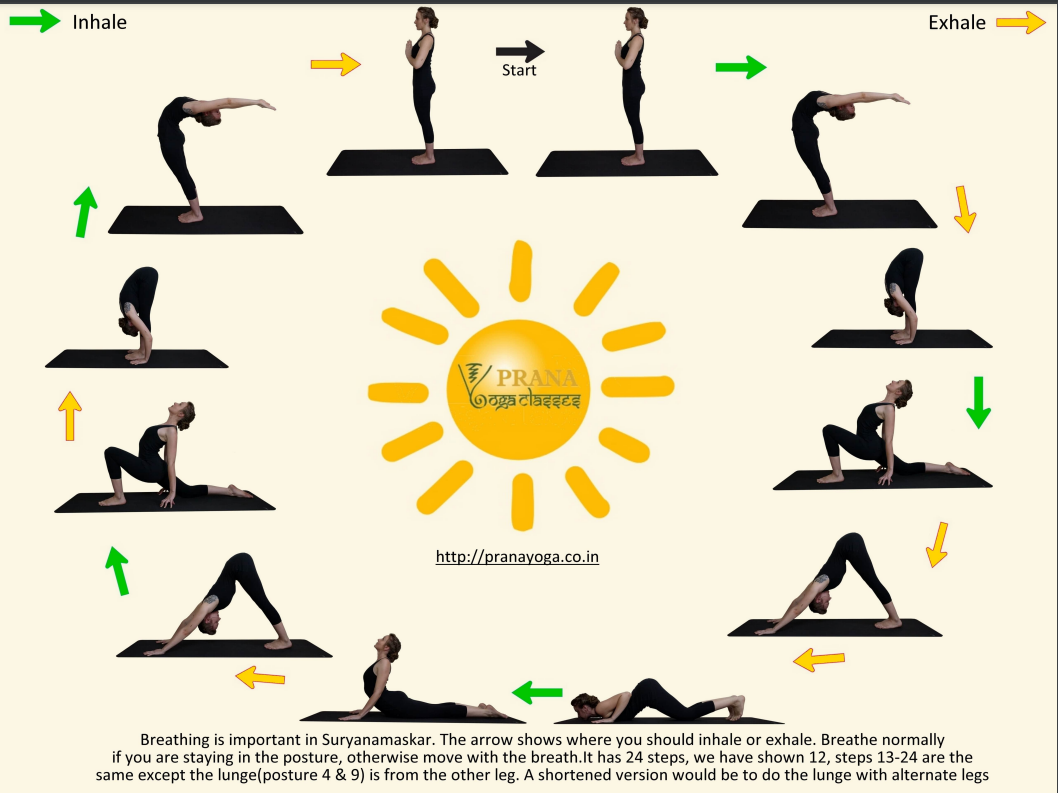
\includegraphics[width=0.8\linewidth,keepaspectratio]{ycb1_suryanamaskar}
        \end{center}	

\end{frame}

%%%%%%%%%%%%%%%%%%%%%%%%%%%%%%%%%%%%%%%%%%%%%%%%%%%%%%%%%%%
\begin{frame}[fragile]\frametitle{Sequence of Surya Namaskara}

        \begin{center}
        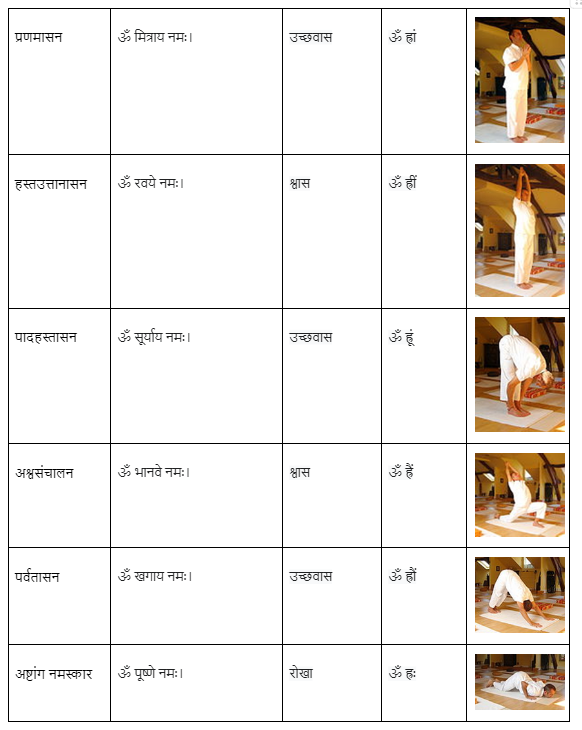
\includegraphics[width=0.5\linewidth,keepaspectratio]{ycb1_sunsal1}
		
        \end{center}	
		

\end{frame}

%%%%%%%%%%%%%%%%%%%%%%%%%%%%%%%%%%%%%%%%%%%%%%%%%%%%%%%%%%%
\begin{frame}[fragile]\frametitle{Sequence of Surya Namaskara}

        \begin{center}
        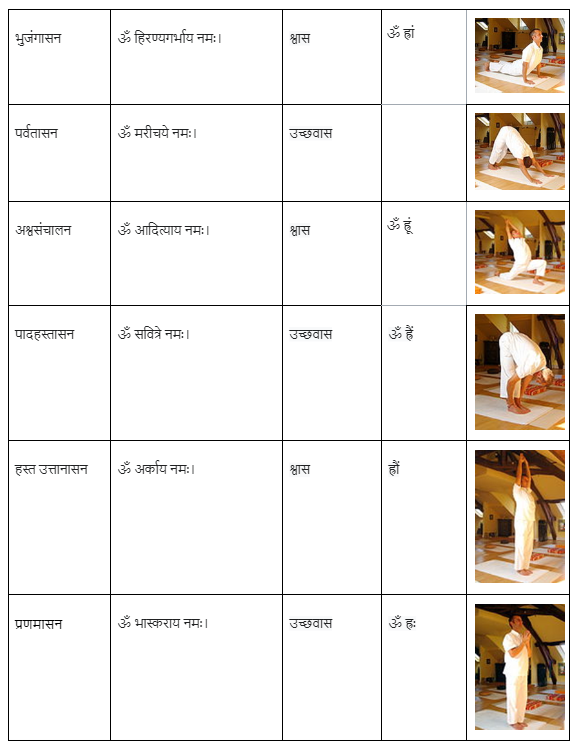
\includegraphics[width=0.5\linewidth,keepaspectratio]{ycb1_sunsal2}
		
		ॐ श्रीसवितृसूर्यनारायणाय नमः।

        \end{center}	

\end{frame}

%%%%%%%%%%%%%%%%%%%%%%%%%%%%%%%%%%%%%%%%%%%%%%%%%%%%%%%%%%%%%%%%%%%%%%%%%%%%%%%%%%
\begin{frame}[fragile]\frametitle{}
\begin{center}
{\Large Yogasana}
\end{center}
\end{frame}

%%%%%%%%%%%%%%%%%%%%%%%%%%%%%%%%%%%%%%%%%%%%%%%%%%%%%%%%%%%%%%%%%%%%%%%%%%%%%%%%%%
\begin{frame}[fragile]\frametitle{Tadasana}
\begin{columns}
    \begin{column}[T]{0.5\linewidth}
      \begin{itemize}
        \item Stand with feet together, arms by sides.
        \item Distribute weight evenly on both feet.
        \item Engage thighs and lift chest.
        \item Extend arms overhead, palms facing each other.
        \item Hold the pose and breathe deeply.
        \item \textbf{Benefits:} Improves posture, strengthens legs, and enhances concentration.
        \item \textbf{Contraindications:} Avoid if you have low blood pressure or are recovering from surgery.
      \end{itemize}
    \end{column}
    \begin{column}[T]{0.5\linewidth}
        \begin{center}
		        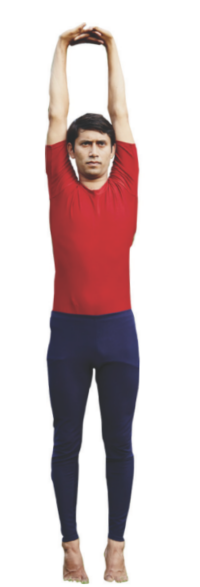
\includegraphics[width=0.35\linewidth,keepaspectratio]{ycb1_tadasan}
				
				{\tiny (Ref: Certification  of Yoga Professionals Official Guidebook For Level I (Instructor))}		
        \end{center}    
    \end{column}
  \end{columns}
\end{frame}

%%%%%%%%%%%%%%%%%%%%%%%%%%%%%%%%%%%%%%%%%%%%%%%%%%%%%%%%%%%%%%%%%%%%%%%%%%%%%%%%%%
\begin{frame}[fragile]\frametitle{Vrikshasana}
\begin{columns}
    \begin{column}[T]{0.5\linewidth}
      \begin{itemize}
        \item Stand in Tadasana position.
        \item Shift weight to one foot, bend the other knee.
        \item Place the sole of the bent foot on the inner thigh of the standing leg.
        \item Join hands in front of the chest or extend overhead.
        \item Hold the position, focus on balance.
        \item \textbf{Benefits:} Enhances balance, strengthens legs, and improves concentration.
        \item \textbf{Contraindications:} Avoid if you have knee or ankle injuries.
      \end{itemize}
    \end{column}
    \begin{column}[T]{0.5\linewidth}
        \begin{center}
		        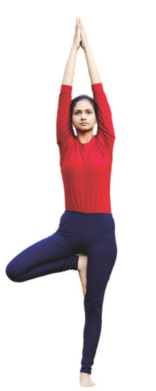
\includegraphics[width=0.4\linewidth,keepaspectratio]{ycb1_vrikshasan}
				
				{\tiny (Ref: Certification  of Yoga Professionals Official Guidebook For Level I (Instructor))}	        
		\end{center}    
    \end{column}
  \end{columns}
\end{frame}

%%%%%%%%%%%%%%%%%%%%%%%%%%%%%%%%%%%%%%%%%%%%%%%%%%%%%%%%%%%%%%%%%%%%%%%%%%%%%%%%%%
\begin{frame}[fragile]\frametitle{Ardha Chakrasana or Hastottanasan}
\begin{columns}
    \begin{column}[T]{0.5\linewidth}
      \begin{itemize}
        \item Stand with feet shoulder-width apart.
        \item Place hands on lower back for support.
        \item Inhale and lift chest, pressing hips forward.
        \item Exhale and gently arch the back.
        \item Hold the pose, breathing deeply.
        \item \textbf{Benefits:} Stretches spine, improves posture, and relieves back pain.
        \item \textbf{Contraindications:} Avoid if you have back injuries or abdominal issues.
      \end{itemize}
    \end{column}
    \begin{column}[T]{0.5\linewidth}
        \begin{center}
        \begin{center}
		        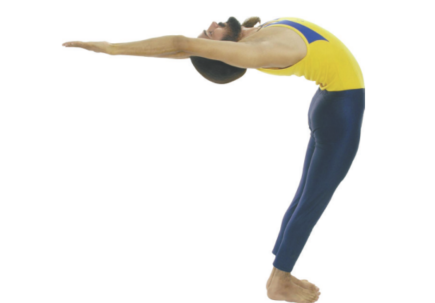
\includegraphics[width=\linewidth,keepaspectratio]{ycb1_ardhachakrasan}
				
				{\tiny (Ref: Certification  of Yoga Professionals Official Guidebook For Level I (Instructor))}	        
		\end{center}   
        \end{center}    
    \end{column}
  \end{columns}
\end{frame}

%%%%%%%%%%%%%%%%%%%%%%%%%%%%%%%%%%%%%%%%%%%%%%%%%%%%%%%%%%%%%%%%%%%%%%%%%%%%%%%%%%
\begin{frame}[fragile]\frametitle{Padahastasana}
\begin{columns}
    \begin{column}[T]{0.5\linewidth}
      \begin{itemize}
        \item Stand with feet together, arms by sides.
        \item Inhale and raise arms overhead.
        \item Exhale and bend forward, reaching for the feet.
        \item Keep knees slightly bent if needed.
        \item Hold the pose and breathe deeply.
        \item \textbf{Benefits:} Stretches hamstrings, improves flexibility, and calms the mind.
        \item \textbf{Contraindications:} Avoid if you have back or hamstring injuries.
      \end{itemize}
    \end{column}
    \begin{column}[T]{0.5\linewidth}
        \begin{center}
        \begin{center}
		        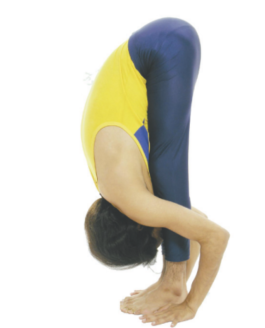
\includegraphics[width=0.9\linewidth,keepaspectratio]{ycb1_padahastasan}
				
				{\tiny (Ref: Certification  of Yoga Professionals Official Guidebook For Level I (Instructor))}	        
		\end{center}   
        \end{center}    
    \end{column}
  \end{columns}
\end{frame}

%%%%%%%%%%%%%%%%%%%%%%%%%%%%%%%%%%%%%%%%%%%%%%%%%%%%%%%%%%%%%%%%%%%%%%%%%%%%%%%%%%
\begin{frame}[fragile]\frametitle{Kati Chakrasana}
\begin{columns}
    \begin{column}[T]{0.5\linewidth}
      \begin{itemize}
        \item Stand with feet shoulder-width apart, arms outstretched.
        \item Twist torso to one side, bringing opposite hand to shoulder.
        \item Hold the twist, then return to center.
        \item Repeat on the other side.
        \item Breathe deeply during each twist.
        \item \textbf{Benefits:} Enhances spinal flexibility, massages abdominal organs, and improves digestion.
        \item \textbf{Contraindications:} Avoid if you have back or spinal issues.
      \end{itemize}
    \end{column}
    \begin{column}[T]{0.5\linewidth}
        \begin{center}
        \begin{center}
		        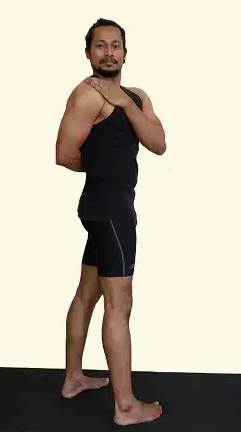
\includegraphics[width=0.6\linewidth,keepaspectratio]{ycb1_katichakrasan}
				
				{\tiny (Ref: Prana Yoga)}	        
		\end{center}   
        \end{center}    
    \end{column}
  \end{columns}
\end{frame}

%%%%%%%%%%%%%%%%%%%%%%%%%%%%%%%%%%%%%%%%%%%%%%%%%%%%%%%%%%%%%%%%%%%%%%%%%%%%%%%%%%
\begin{frame}[fragile]\frametitle{Trikonasana}
\begin{columns}
    \begin{column}[T]{0.5\linewidth}
      \begin{itemize}
        \item Stand with feet wide apart, arms extended.
        \item Turn one foot out and the other foot slightly in.
        \item Reach towards the foot, placing hand on ankle or shin.
        \item Extend the other arm upwards, gaze up.
        \item Hold the position, then switch sides.
        \item \textbf{Benefits:} Stretches legs, improves balance, and strengthens core.
        \item \textbf{Contraindications:} Avoid if you have leg or back injuries.
      \end{itemize}
    \end{column}
    \begin{column}[T]{0.5\linewidth}
        \begin{center}
        \begin{center}
		        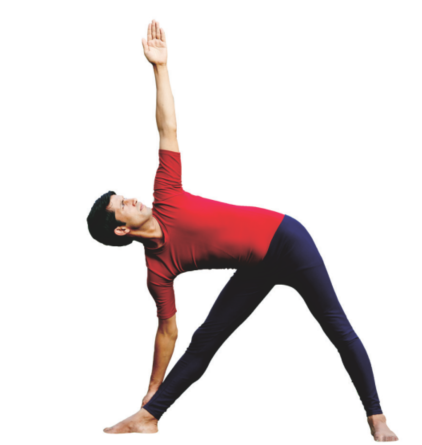
\includegraphics[width=\linewidth,keepaspectratio]{ycb1_trikonasan}
				
				{\tiny (Ref: Certification  of Yoga Professionals Official Guidebook For Level I (Instructor))}	        
		\end{center}   
        \end{center}    
    \end{column}
  \end{columns}
\end{frame}

%%%%%%%%%%%%%%%%%%%%%%%%%%%%%%%%%%%%%%%%%%%%%%%%%%%%%%%%%%%%%%%%%%%%%%%%%%%%%%%%%%
\begin{frame}[fragile]\frametitle{Dandasana}
\begin{columns}
    \begin{column}[T]{0.5\linewidth}
      \begin{itemize}
        \item Sit with legs extended, feet flexed.
        \item Keep spine straight and shoulders relaxed.
        \item Place hands beside hips, fingers pointing forward.
        \item Engage thigh muscles and lift chest.
        \item Hold the pose, breathing steadily.
        \item \textbf{Benefits:} Strengthens back and legs, improves posture, and calms the mind.
        \item \textbf{Contraindications:} Avoid if you have lower back pain or hamstring injuries.
      \end{itemize}
    \end{column}
    \begin{column}[T]{0.5\linewidth}
        \begin{center}
        \begin{center}
		        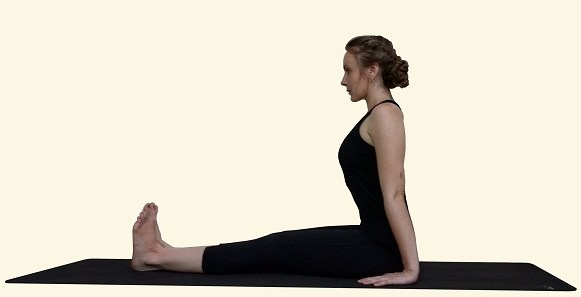
\includegraphics[width=\linewidth,keepaspectratio]{ycb1_dandasan}
				
				{\tiny (Ref: Prana Yoga)}	        
		\end{center}   
        \end{center}    
    \end{column}
  \end{columns}
\end{frame}

%%%%%%%%%%%%%%%%%%%%%%%%%%%%%%%%%%%%%%%%%%%%%%%%%%%%%%%%%%%%%%%%%%%%%%%%%%%%%%%%%%
\begin{frame}[fragile]\frametitle{Sukhasana}
\begin{columns}
    \begin{column}[T]{0.5\linewidth}
      \begin{itemize}
        \item Sit with legs crossed comfortably.
        \item Place hands on knees or in a mudra.
        \item Keep spine upright and shoulders relaxed.
        \item Close eyes and focus on breath.
        \item Hold the position, breathing deeply.
        \item \textbf{Benefits:} Promotes relaxation, improves flexibility, and calms the mind.
        \item \textbf{Contraindications:} Avoid if you have knee or hip injuries.
      \end{itemize}
    \end{column}
    \begin{column}[T]{0.5\linewidth}
        \begin{center}
        \begin{center}
		        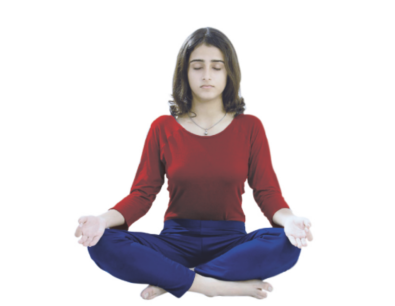
\includegraphics[width=\linewidth,keepaspectratio]{ycb1_sukhasan}
				
				{\tiny (Ref: Certification  of Yoga Professionals Official Guidebook For Level I (Instructor))}	        
		\end{center}   
        \end{center}    
    \end{column}
  \end{columns}
\end{frame}

%%%%%%%%%%%%%%%%%%%%%%%%%%%%%%%%%%%%%%%%%%%%%%%%%%%%%%%%%%%%%%%%%%%%%%%%%%%%%%%%%%
\begin{frame}[fragile]\frametitle{Padmasana}
\begin{columns}
    \begin{column}[T]{0.5\linewidth}
      \begin{itemize}
        \item Sit with legs extended, then bend one knee.
        \item Place the foot on the opposite thigh.
        \item Repeat with the other leg, placing the foot on the opposite thigh.
        \item Keep spine straight and shoulders relaxed.
        \item Hold the position, focusing on breath.
        \item \textbf{Benefits:} Enhances meditation, stretches hips, and calms the mind.
        \item \textbf{Contraindications:} Avoid if you have knee or hip injuries.
      \end{itemize}
    \end{column}
    \begin{column}[T]{0.5\linewidth}
        \begin{center}
        \begin{center}
		        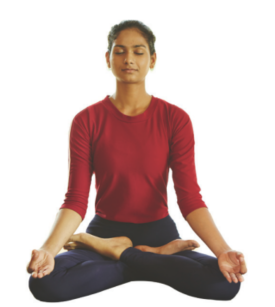
\includegraphics[width=\linewidth,keepaspectratio]{ycb1_padmasan}
				
				{\tiny (Ref: Certification  of Yoga Professionals Official Guidebook For Level I (Instructor))}	        
		\end{center}   
        \end{center}    
    \end{column}
  \end{columns}
\end{frame}

%%%%%%%%%%%%%%%%%%%%%%%%%%%%%%%%%%%%%%%%%%%%%%%%%%%%%%%%%%%%%%%%%%%%%%%%%%%%%%%%%%
\begin{frame}[fragile]\frametitle{Vajrasana}
\begin{columns}
    \begin{column}[T]{0.5\linewidth}
      \begin{itemize}
        \item Kneel on the floor, sit back on heels.
        \item Keep thighs perpendicular to the floor.
        \item Place hands on knees, palms facing down.
        \item Keep spine straight and shoulders relaxed.
        \item Breathe deeply, holding the position.
        \item \textbf{Benefits:} Aids digestion, relieves lower back pain, and improves posture.
        \item \textbf{Contraindications:} Avoid if you have knee or ankle injuries.
      \end{itemize}
    \end{column}
    \begin{column}[T]{0.5\linewidth}
        \begin{center}
        \begin{center}
		        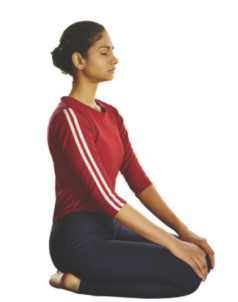
\includegraphics[width=0.8\linewidth,keepaspectratio]{ycb1_vajrasan}
				
				{\tiny (Ref: Certification  of Yoga Professionals Official Guidebook For Level I (Instructor))}	        
		\end{center}   
        \end{center}    
    \end{column}
  \end{columns}
\end{frame}

%%%%%%%%%%%%%%%%%%%%%%%%%%%%%%%%%%%%%%%%%%%%%%%%%%%%%%%%%%%%%%%%%%%%%%%%%%%%%%%%%%
\begin{frame}[fragile]\frametitle{Bhadrasana}
\begin{columns}
    \begin{column}[T]{0.5\linewidth}
      \begin{itemize}
        \item Sit with legs extended, then bend knees and bring feet together.
        \item Place feet close to the pelvis, holding toes with hands.
        \item Press knees gently towards the floor.
        \item Keep spine erect and shoulders relaxed.
        \item Hold the pose and breathe deeply.
        \item \textbf{Benefits:} Opens hips, improves flexibility, and calms the mind.
        \item \textbf{Contraindications:} Avoid if you have knee or hip injuries.
      \end{itemize}
    \end{column}
    \begin{column}[T]{0.5\linewidth}
        \begin{center}
        \begin{center}
		        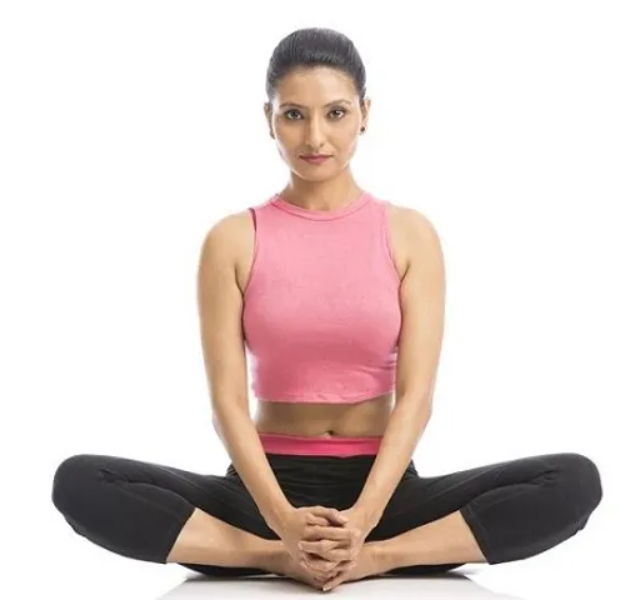
\includegraphics[width=\linewidth,keepaspectratio]{ycb1_bhadrasan}
				
				{\tiny (Ref: Patanjali Japan Foundation)}	        
		\end{center}   
        \end{center}    
    \end{column}
  \end{columns}
\end{frame}

%%%%%%%%%%%%%%%%%%%%%%%%%%%%%%%%%%%%%%%%%%%%%%%%%%%%%%%%%%%%%%%%%%%%%%%%%%%%%%%%%%
\begin{frame}[fragile]\frametitle{Mandukasana}
\begin{columns}
    \begin{column}[T]{0.5\linewidth}
      \begin{itemize}
        \item Start in a kneeling position, sit on heels.
        \item Place palms together in front of the chest.
        \item Inhale and stretch arms forward, keeping palms together.
        \item Exhale and bring hands back to the chest.
        \item Repeat the sequence.
        \item \textbf{Benefits:} Improves flexibility of hips and thighs, enhances focus.
        \item \textbf{Contraindications:} Avoid if you have knee or back issues.
      \end{itemize}
    \end{column}
    \begin{column}[T]{0.5\linewidth}
        \begin{center}
        \begin{center}
		        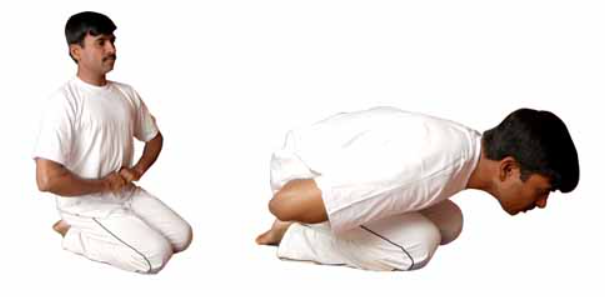
\includegraphics[width=\linewidth,keepaspectratio]{ycb1_mandukasan}
				
				{\tiny (Ref: Atma Bodh)}	        
		\end{center}   
        \end{center}    
    \end{column}
  \end{columns}
\end{frame}

%%%%%%%%%%%%%%%%%%%%%%%%%%%%%%%%%%%%%%%%%%%%%%%%%%%%%%%%%%%%%%%%%%%%%%%%%%%%%%%%%%
\begin{frame}[fragile]\frametitle{Ushtrasana}
\begin{columns}
    \begin{column}[T]{0.5\linewidth}
      \begin{itemize}
        \item Kneel with knees hip-width apart.
        \item Place hands on lower back for support.
        \item Inhale and lift chest, arching back.
        \item Reach for heels with hands, if possible.
        \item Hold the position, breathing deeply.
        \item \textbf{Benefits:} Stretches the entire front body, opens chest, and improves posture.
        \item \textbf{Contraindications:} Avoid if you have back or neck issues.
      \end{itemize}
    \end{column}
    \begin{column}[T]{0.5\linewidth}
        \begin{center}
        \begin{center}
		        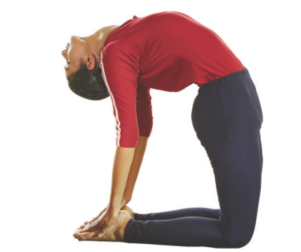
\includegraphics[width=\linewidth,keepaspectratio]{ycb1_ushtrasan}
				
				{\tiny (Ref: Certification  of Yoga Professionals Official Guidebook For Level I (Instructor))}	        
		\end{center}   
        \end{center}    
    \end{column}
  \end{columns}
\end{frame}

%%%%%%%%%%%%%%%%%%%%%%%%%%%%%%%%%%%%%%%%%%%%%%%%%%%%%%%%%%%%%%%%%%%%%%%%%%%%%%%%%%
\begin{frame}[fragile]\frametitle{Shashankasana}
\begin{columns}
    \begin{column}[T]{0.5\linewidth}
      \begin{itemize}
        \item Kneel and sit on heels.
        \item Extend arms forward on the floor.
        \item Rest forehead on the ground.
        \item Hold the position, breathing deeply.
        \item \textbf{Benefits:} Relieves stress, stretches back and thighs.
        \item \textbf{Contraindications:} Avoid if you have knee or back injuries.
      \end{itemize}
    \end{column}
    \begin{column}[T]{0.5\linewidth}
        \begin{center}
        \begin{center}
		        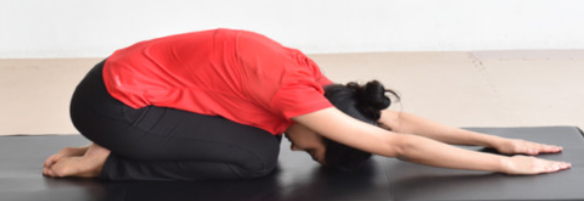
\includegraphics[width=\linewidth,keepaspectratio]{ycb1_shashankasan}
				
				{\tiny (Ref: Certification  of Yoga Professionals Official Guidebook For Level I (Instructor))}	        
		\end{center}   
        \end{center}    
    \end{column}
  \end{columns}
\end{frame}

%%%%%%%%%%%%%%%%%%%%%%%%%%%%%%%%%%%%%%%%%%%%%%%%%%%%%%%%%%%%%%%%%%%%%%%%%%%%%%%%%%
\begin{frame}[fragile]\frametitle{Uttana Mandukasana}
\begin{columns}
    \begin{column}[T]{0.5\linewidth}
      \begin{itemize}
        \item Start in Mandukasana position.
        \item Bend forward from hips, extending arms forward.
        \item Rest forehead on the floor, keep arms extended.
        \item Hold the position, breathing deeply.
        \item \textbf{Benefits:} Enhances spinal flexibility, stretches back and thighs.
        \item \textbf{Contraindications:} Avoid if you have knee or back injuries.
      \end{itemize}
    \end{column}
    \begin{column}[T]{0.5\linewidth}
        \begin{center}
        \begin{center}
		        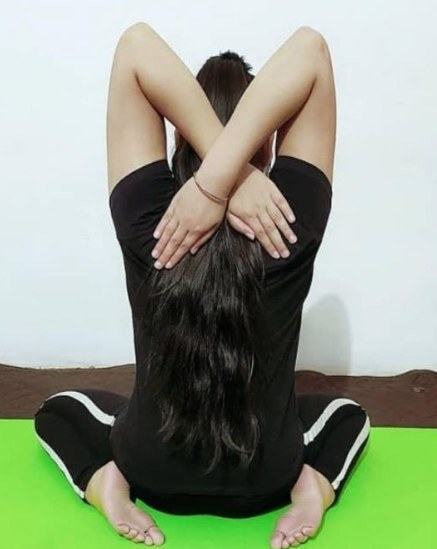
\includegraphics[width=0.9\linewidth,keepaspectratio]{ycb1_uttanamandukasan}
				
				{\tiny (Ref: Certification  of Yoga Professionals Official Guidebook For Level I (Instructor))}	        
		\end{center}   
        \end{center}    
    \end{column}
  \end{columns}
\end{frame}

%%%%%%%%%%%%%%%%%%%%%%%%%%%%%%%%%%%%%%%%%%%%%%%%%%%%%%%%%%%%%%%%%%%%%%%%%%%%%%%%%%
\begin{frame}[fragile]\frametitle{Paschimottanasana}
\begin{columns}
    \begin{column}[T]{0.5\linewidth}
      \begin{itemize}
        \item Sit with legs extended, feet flexed.
        \item Inhale and lengthen spine.
        \item Exhale and bend forward, reaching for feet.
        \item Hold the pose and breathe deeply.
        \item \textbf{Benefits:} Stretches the spine and hamstrings, calms the mind.
        \item \textbf{Contraindications:} Avoid if you have back or hamstring injuries.
      \end{itemize}
    \end{column}
    \begin{column}[T]{0.5\linewidth}
        \begin{center}
        \begin{center}
		        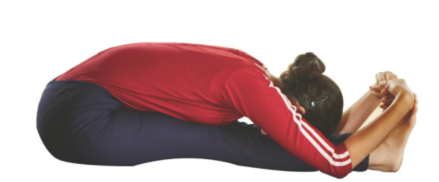
\includegraphics[width=\linewidth,keepaspectratio]{ycb1_pashchimottansasan}
				
				{\tiny (Ref: Certification  of Yoga Professionals Official Guidebook For Level I (Instructor))}	        
		\end{center}   
        \end{center}    
    \end{column}
  \end{columns}
\end{frame}

%%%%%%%%%%%%%%%%%%%%%%%%%%%%%%%%%%%%%%%%%%%%%%%%%%%%%%%%%%%%%%%%%%%%%%%%%%%%%%%%%%
\begin{frame}[fragile]\frametitle{Purvottanasana}
\begin{columns}
    \begin{column}[T]{0.5\linewidth}
      \begin{itemize}
        \item Sit with legs extended and hands behind hips.
        \item Inhale and lift hips off the floor, pressing palms into the ground.
        \item Open chest and face upward.
        \item Hold the pose and breathe deeply.
        \item \textbf{Benefits:} Strengthens arms and shoulders, stretches chest and front body.
        \item \textbf{Contraindications:} Avoid if you have wrist or shoulder injuries.
      \end{itemize}
    \end{column}
    \begin{column}[T]{0.5\linewidth}
        \begin{center}
        \begin{center}
		        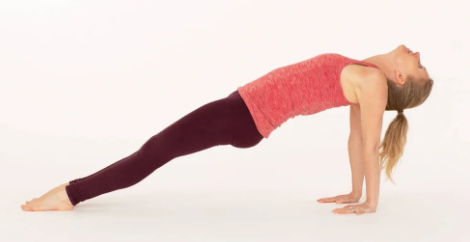
\includegraphics[width=\linewidth,keepaspectratio]{ycb1_purvottansasan}
				
				{\tiny (Ref: Ekhart Yoga)}	        
		\end{center}   
        \end{center}    
    \end{column}
  \end{columns}
\end{frame}

%%%%%%%%%%%%%%%%%%%%%%%%%%%%%%%%%%%%%%%%%%%%%%%%%%%%%%%%%%%%%%%%%%%%%%%%%%%%%%%%%%
\begin{frame}[fragile]\frametitle{Vakrasana}
\begin{columns}
    \begin{column}[T]{0.5\linewidth}
      \begin{itemize}
        \item Sit with legs extended and back straight.
        \item Bend one knee and place the foot on the outside of the opposite thigh.
        \item Twist torso towards the bent knee, placing the opposite elbow on the knee.
        \item Hold the twist, then switch sides.
        \item \textbf{Benefits:} Enhances spinal flexibility, massages abdominal organs.
        \item \textbf{Contraindications:} Avoid if you have spinal or abdominal issues.
      \end{itemize}
    \end{column}
    \begin{column}[T]{0.5\linewidth}
        \begin{center}
        \begin{center}
		        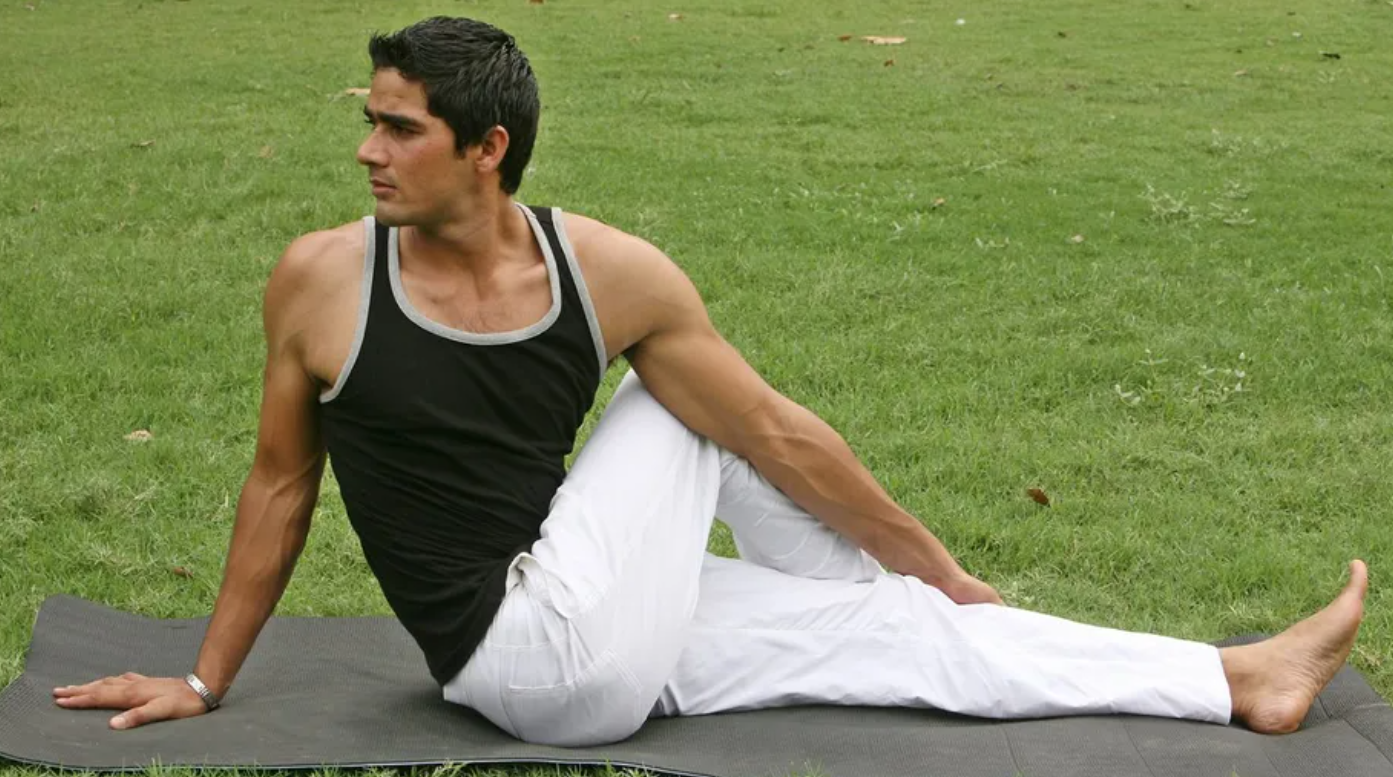
\includegraphics[width=\linewidth,keepaspectratio]{ycb1_vakrasan}
				
				{\tiny (Ref: CONDE NAST TRAVELLER)}	        
		\end{center}   
        \end{center}    
    \end{column}
  \end{columns}
\end{frame}

%%%%%%%%%%%%%%%%%%%%%%%%%%%%%%%%%%%%%%%%%%%%%%%%%%%%%%%%%%%%%%%%%%%%%%%%%%%%%%%%%%
\begin{frame}[fragile]\frametitle{Gomukhasana}
\begin{columns}
    \begin{column}[T]{0.5\linewidth}
      \begin{itemize}
        \item Sit with legs crossed, one knee stacked on top of the other.
        \item Bring one arm behind the back, and the other arm over the shoulder.
        \item Join hands behind the back if possible.
        \item Hold the pose and breathe deeply.
        \item \textbf{Benefits:} Stretches shoulders, hips, and thighs.
        \item \textbf{Contraindications:} Avoid if you have shoulder or knee injuries.
      \end{itemize}
    \end{column}
    \begin{column}[T]{0.5\linewidth}
        \begin{center}
        \begin{center}
		        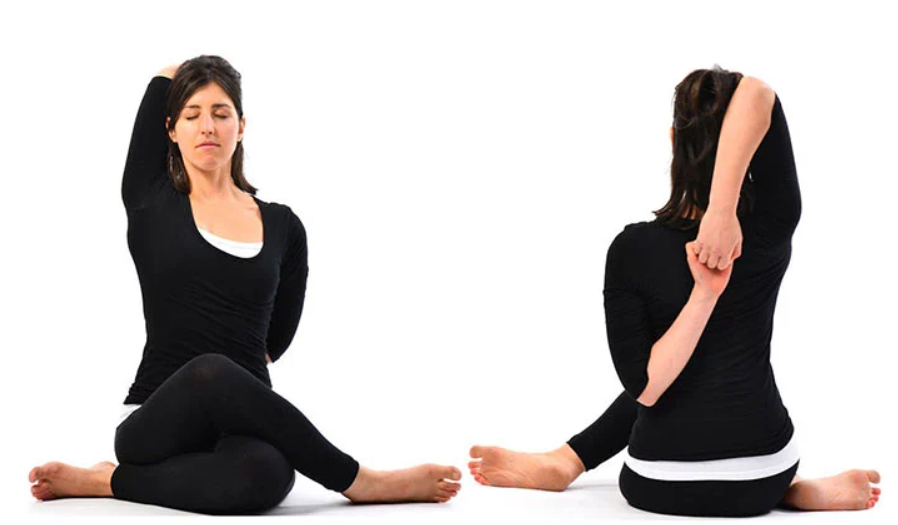
\includegraphics[width=\linewidth,keepaspectratio]{ycb1_gomukhasan}
				
				{\tiny (Ref: Himalayan Yoga Ashram)}	        
		\end{center}   
        \end{center}    
    \end{column}
  \end{columns}
\end{frame}

%%%%%%%%%%%%%%%%%%%%%%%%%%%%%%%%%%%%%%%%%%%%%%%%%%%%%%%%%%%%%%%%%%%%%%%%%%%%%%%%%%
\begin{frame}[fragile]\frametitle{Bhujangasana}
\begin{columns}
    \begin{column}[T]{0.5\linewidth}
      \begin{itemize}
        \item Lie on your stomach, legs extended, and feet together.
        \item Place hands under shoulders, elbows close to the body.
        \item Inhale and lift chest, keeping the navel on the floor.
        \item Hold the pose and breathe deeply.
        \item \textbf{Benefits:} Strengthens back, stretches chest and shoulders.
        \item \textbf{Contraindications:} Avoid if you have back or wrist injuries.
      \end{itemize}
    \end{column}
    \begin{column}[T]{0.5\linewidth}
        \begin{center}
        \begin{center}
		        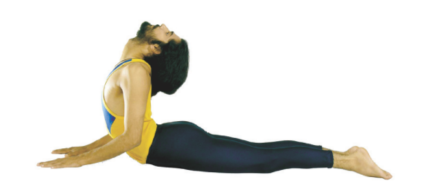
\includegraphics[width=\linewidth,keepaspectratio]{ycb1_bhujangasan}
				
				{\tiny (Ref: Certification  of Yoga Professionals Official Guidebook For Level I (Instructor))}	        
		\end{center}   
        \end{center}    
    \end{column}
  \end{columns}
\end{frame}

%%%%%%%%%%%%%%%%%%%%%%%%%%%%%%%%%%%%%%%%%%%%%%%%%%%%%%%%%%%%%%%%%%%%%%%%%%%%%%%%%%
\begin{frame}[fragile]\frametitle{Shalabhasana}
\begin{columns}
    \begin{column}[T]{0.5\linewidth}
      \begin{itemize}
        \item Lie on your stomach, arms by sides.
        \item Inhale and lift legs and chest off the floor.
        \item Keep arms and feet active.
        \item Hold the position, breathing deeply.
        \item \textbf{Benefits:} Strengthens lower back, improves posture.
        \item \textbf{Contraindications:} Avoid if you have back or abdominal issues.
      \end{itemize}
    \end{column}
    \begin{column}[T]{0.5\linewidth}
        \begin{center}
        \begin{center}
		        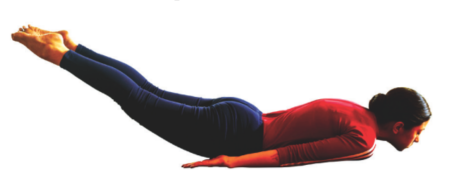
\includegraphics[width=\linewidth,keepaspectratio]{ycb1_shalabhasan}
				
				{\tiny (Ref: Certification  of Yoga Professionals Official Guidebook For Level I (Instructor))}	        
		\end{center}   
        \end{center}    
    \end{column}
  \end{columns}
\end{frame}

%%%%%%%%%%%%%%%%%%%%%%%%%%%%%%%%%%%%%%%%%%%%%%%%%%%%%%%%%%%%%%%%%%%%%%%%%%%%%%%%%%
\begin{frame}[fragile]\frametitle{Makarasana}
\begin{columns}
    \begin{column}[T]{0.5\linewidth}
      \begin{itemize}
        \item Lie on your stomach, arms extended to sides.
        \item Bend knees and place feet on the floor.
        \item Rest forehead on the hands or ground.
        \item Breathe deeply and relax.
        \item \textbf{Benefits:} Relieves back pain, relaxes spine.
        \item \textbf{Contraindications:} None.
      \end{itemize}
    \end{column}
    \begin{column}[T]{0.5\linewidth}
        \begin{center}
        \begin{center}
		        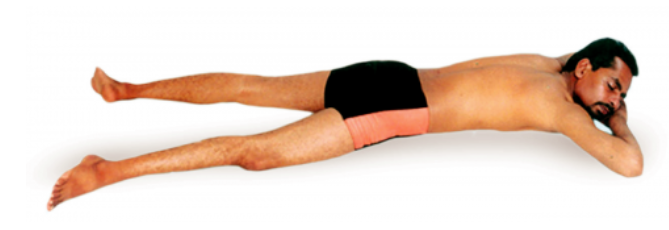
\includegraphics[width=\linewidth,keepaspectratio]{ycb1_makarasan}
				
				{\tiny (Ref: Vydya Health)}	        
		\end{center}   
        \end{center}    
    \end{column}
  \end{columns}
\end{frame}

%%%%%%%%%%%%%%%%%%%%%%%%%%%%%%%%%%%%%%%%%%%%%%%%%%%%%%%%%%%%%%%%%%%%%%%%%%%%%%%%%%
\begin{frame}[fragile]\frametitle{Pavanamuktasana}
\begin{columns}
    \begin{column}[T]{0.5\linewidth}
      \begin{itemize}
        \item Lie on your back, knees bent, and feet on the floor.
        \item Hug knees to chest, interlace fingers around shins.
        \item Lift head and shoulders off the floor.
        \item Hold the position and breathe deeply.
        \item \textbf{Benefits:} Relieves gas, massages abdominal organs.
        \item \textbf{Contraindications:} Avoid if you have back issues or are pregnant.
      \end{itemize}
    \end{column}
    \begin{column}[T]{0.5\linewidth}
        \begin{center}
        \begin{center}
		        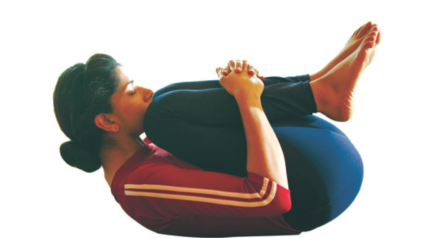
\includegraphics[width=\linewidth,keepaspectratio]{ycb1_pavanamuktasan}
				
				{\tiny (Ref: Certification  of Yoga Professionals Official Guidebook For Level I (Instructor))}	        
		\end{center}   
        \end{center}    
    \end{column}
  \end{columns}
\end{frame}

%%%%%%%%%%%%%%%%%%%%%%%%%%%%%%%%%%%%%%%%%%%%%%%%%%%%%%%%%%%%%%%%%%%%%%%%%%%%%%%%%%
\begin{frame}[fragile]\frametitle{Uttanapadasana / Ardha Halasana}
\begin{columns}
    \begin{column}[T]{0.5\linewidth}
      \begin{itemize}
        \item Lie on your back, legs extended, and arms by sides.
        \item Inhale and lift legs to a 45-degree angle.
        \item Keep back and shoulders on the floor.
        \item Hold the position and breathe deeply.
        \item \textbf{Benefits:} Strengthens abdominal muscles, tones legs.
        \item \textbf{Contraindications:} Avoid if you have back or leg issues.
      \end{itemize}
    \end{column}
    \begin{column}[T]{0.5\linewidth}
        \begin{center}
        \begin{center}
		        \includegraphics[width=\linewidth,keepaspectratio]{ycb1_uttanpadasan}
				
				{\tiny (Ref: Bodhi School of Yoga)}	        
		\end{center}   
        \end{center}    
    \end{column}
  \end{columns}
\end{frame}

% %%%%%%%%%%%%%%%%%%%%%%%%%%%%%%%%%%%%%%%%%%%%%%%%%%%%%%%%%%%%%%%%%%%%%%%%%%%%%%%%%%
% \begin{frame}[fragile]\frametitle{}
% \begin{columns}
    % \begin{column}[T]{0.5\linewidth}
      % \begin{itemize}
        % \item Lie on your back, arms by sides.
        % \item Lift legs overhead, bringing toes to the floor behind the head.
        % \item Support lower back with hands if needed.
        % \item Hold the position and breathe deeply.
        % \item \textbf{Benefits:} Stretches back and legs, strengthens core.
        % \item \textbf{Contraindications:} Avoid if you have neck or back issues.
      % \end{itemize}
    % \end{column}
    % \begin{column}[T]{0.5\linewidth}
        % \begin{center}
        % \begin{center}
		        % \includegraphics[width=\linewidth,keepaspectratio]{ycb1_vrikshasan}
				
				% {\tiny (Ref: Certification  of Yoga Professionals Official Guidebook For Level I (Instructor))}	        
		% \end{center}   
        % \end{center}    
    % \end{column}
  % \end{columns}
% \end{frame}

%%%%%%%%%%%%%%%%%%%%%%%%%%%%%%%%%%%%%%%%%%%%%%%%%%%%%%%%%%%%%%%%%%%%%%%%%%%%%%%%%%
\begin{frame}[fragile]\frametitle{Setubandhasana}
\begin{columns}
    \begin{column}[T]{0.5\linewidth}
      \begin{itemize}
        \item Lie on your back, knees bent, feet on the floor.
        \item Lift hips towards the ceiling, pressing into feet.
        \item Interlace fingers under back for support.
        \item Hold the position and breathe deeply.
        \item \textbf{Benefits:} Strengthens back and legs, stretches chest.
        \item \textbf{Contraindications:} Avoid if you have neck or back injuries.
      \end{itemize}
    \end{column}
    \begin{column}[T]{0.5\linewidth}
        \begin{center}
        \begin{center}
		        \includegraphics[width=\linewidth,keepaspectratio]{ycb1_setubandhasan}
				
				{\tiny (Ref: Rishikesh Yogis Yogashala)}	        
		\end{center}   
        \end{center}    
    \end{column}
  \end{columns}
\end{frame}

%%%%%%%%%%%%%%%%%%%%%%%%%%%%%%%%%%%%%%%%%%%%%%%%%%%%%%%%%%%%%%%%%%%%%%%%%%%%%%%%%%
\begin{frame}[fragile]\frametitle{Vipareetakarani}
\begin{columns}
    \begin{column}[T]{0.5\linewidth}
      \begin{itemize}
        \item Lie on your back, legs extended.
        \item Lift legs and hips towards the ceiling.
        \item Support lower back with hands if needed.
        \item Keep shoulders and neck relaxed on the floor.
        \item Hold the position and breathe deeply.
        \item \textbf{Benefits:} Improves circulation, reduces stress.
        \item \textbf{Contraindications:} Avoid if you have neck or back issues.
      \end{itemize}
    \end{column}
    \begin{column}[T]{0.5\linewidth}
        \begin{center}
        \begin{center}
		        \includegraphics[width=\linewidth,keepaspectratio]{ycb1_vipartikarni}
				
				{\tiny (Ref: Yoga4Lyf)}	        
		\end{center}   
        \end{center}    
    \end{column}
  \end{columns}
\end{frame}

%%%%%%%%%%%%%%%%%%%%%%%%%%%%%%%%%%%%%%%%%%%%%%%%%%%%%%%%%%%%%%%%%%%%%%%%%%%%%%%%%%
\begin{frame}[fragile]\frametitle{Saral Matsyasana}
\begin{columns}
    \begin{column}[T]{0.5\linewidth}
      \begin{itemize}
        \item Lie on your back, legs extended.
        \item Place hands under hips for support.
        \item Lift chest and head, arching back.
        \item Keep elbows close to the floor, shoulders relaxed.
        \item Hold the position and breathe deeply.
        \item \textbf{Benefits:} Stretches chest and neck, improves posture.
        \item \textbf{Contraindications:} Avoid if you have neck or back injuries.
      \end{itemize}
    \end{column}
    \begin{column}[T]{0.5\linewidth}
        \begin{center}
        \begin{center}
		        \includegraphics[width=\linewidth,keepaspectratio]{ycb1_saralmatsyasan}
				
				{\tiny (Ref: Kerala Tourism)}	        
		\end{center}   
        \end{center}    
    \end{column}
  \end{columns}
\end{frame}




%%%%%%%%%%%%%%%%%%%%%%%%%%%%%%%%%%%%%%%%%%%%%%%%%%%%%%%%%%%%%%%%%%%%%%%%%%%%%%%%%%
\begin{frame}[fragile]\frametitle{}
\begin{center}
{\Large Preparatory Breathing Practices }
\end{center}
\end{frame}

%%%%%%%%%%%%%%%%%%%%%%%%%%%%%%%%%%%%%%%%%%%%%%%%%%%%%%%%%%%
\begin{frame}[fragile]\frametitle{Preparatory Breathing Practices: Overview}
      \begin{itemize}
        \item \textbf{Preparatory Breathing}: Essential for \textbf{effective practice}.
        \item Prepares the body for \textbf{deeper} and \textbf{advanced} breathing techniques.
        \item Helps in \textbf{calming} the \textbf{mind} and \textbf{focusing} attention.
        \item Improves \textbf{lung capacity} and \textbf{respiratory function}.
        \item Integrates with \textbf{asanas} for \textbf{enhanced practice}.
      \end{itemize}

\end{frame}

%%%%%%%%%%%%%%%%%%%%%%%%%%%%%%%%%%%%%%%%%%%%%%%%%%%%%%%%%%%
\begin{frame}[fragile]\frametitle{Abdominal Breathing (Diaphragmatic Breathing)}
\begin{columns}
    \begin{column}[T]{0.5\linewidth}
      \begin{itemize}
        \item Focuses on \textbf{diaphragm} movement.
        \item \textbf{Inhale} deeply through the nose, expanding the \textbf{abdomen}.
        \item \textbf{Exhale} slowly through the mouth, contracting the \textbf{abdomen}.
        \item Promotes \textbf{relaxation} and \textbf{stress relief}.
        \item Enhances \textbf{oxygenation} and \textbf{lung efficiency}.
      \end{itemize}
    \end{column}
    \begin{column}[T]{0.5\linewidth}
        \begin{center}
        \includegraphics[width=\linewidth,keepaspectratio]{ycb1_abdominalbreathing}
				
		{\tiny (Ref: Certification  of Yoga Professionals Official Guidebook For Level I (Instructor))}	  		
        \end{center}	
    \end{column}
\end{columns}
\end{frame}

%%%%%%%%%%%%%%%%%%%%%%%%%%%%%%%%%%%%%%%%%%%%%%%%%%%%%%%%%%%
\begin{frame}[fragile]\frametitle{Chest Breathing}
\begin{columns}
    \begin{column}[T]{0.5\linewidth}
      \begin{itemize}
        \item Involves the \textbf{chest} and \textbf{intercostal muscles}.
        \item \textbf{Inhale} to expand the \textbf{chest} and \textbf{rib cage}.
        \item \textbf{Exhale} to contract the \textbf{chest}.
        \item Useful for \textbf{increasing} lung capacity.
        \item Often combined with \textbf{abdominal breathing} for balance.
      \end{itemize}
    \end{column}
    \begin{column}[T]{0.5\linewidth}
        \begin{center}
        \includegraphics[width=\linewidth,keepaspectratio]{ycb1_chestbreathing}
				
		{\tiny (Ref: Certification  of Yoga Professionals Official Guidebook For Level I (Instructor))}	  
        \end{center}	
    \end{column}
\end{columns}
\end{frame}

%%%%%%%%%%%%%%%%%%%%%%%%%%%%%%%%%%%%%%%%%%%%%%%%%%%%%%%%%%%
\begin{frame}[fragile]\frametitle{Clavicular Breathing}
\begin{columns}
    \begin{column}[T]{0.5\linewidth}
      \begin{itemize}
        \item Focuses on \textbf{upper chest} and \textbf{collarbone}.
        \item \textbf{Inhale} to lift the \textbf{clavicles} and expand the \textbf{upper chest}.
        \item \textbf{Exhale} to lower the \textbf{clavicles}.
        \item Helps in \textbf{expanding lung capacity}.
        \item Often used in conjunction with other \textbf{breathing techniques}.
      \end{itemize}
    \end{column}
    \begin{column}[T]{0.5\linewidth}
        \begin{center}
        \includegraphics[width=\linewidth,keepaspectratio]{ycb1_clavicularbreathing}
				
		{\tiny (Ref: Sri Sri School of Yoga)}	  
        \end{center}	
    \end{column}
\end{columns}
\end{frame}

%%%%%%%%%%%%%%%%%%%%%%%%%%%%%%%%%%%%%%%%%%%%%%%%%%%%%%%%%%%
\begin{frame}[fragile]\frametitle{Combination Breathing (Three-Part Breathing)}
\begin{columns}
    \begin{column}[T]{0.5\linewidth}
      \begin{itemize}
        \item Combines \textbf{abdominal}, \textbf{chest}, and \textbf{clavicular} breathing.
        \item \textbf{Inhale} first into the abdomen, then the chest, and finally the clavicles.
        \item \textbf{Exhale} in reverse order.
        \item Enhances \textbf{complete lung expansion}.
        \item Provides a \textbf{holistic} breathing experience.
      \end{itemize}
    \end{column}
    \begin{column}[T]{0.5\linewidth}
        \begin{center}
        \includegraphics[width=\linewidth,keepaspectratio]{ycb1_threepartbreathing}
				
		{\tiny (Ref: Beginner Yoga Flow)}	  
        \end{center}	
    \end{column}
\end{columns}
\end{frame}


%%%%%%%%%%%%%%%%%%%%%%%%%%%%%%%%%%%%%%%%%%%%%%%%%%%%%%%%%%%%%%%%%%%%%%%%%%%%%%%%%%
\begin{frame}[fragile]\frametitle{}
\begin{center}
{\Large Pranayama}
\end{center}
\end{frame}

%%%%%%%%%%%%%%%%%%%%%%%%%%%%%%%%%%%%%%%%%%%%%%%%%%%%%%%%%%%
\begin{frame}[fragile]\frametitle{Pranayama: Concept}

      \begin{itemize}
        \item \textbf{Pranayama}: Control of \textbf{breath}.
        \item Derived from \textbf{Sanskrit}, meaning \textbf{extension} of \textbf{life force}.
        \item Essential for \textbf{mental} and \textbf{physical health}.
        \item Regulates \textbf{energy flow} and \textbf{calms the mind}.
        \item Integrates with \textbf{asana} for \textbf{holistic practice}.
		\item  यम, नियम, आसन, प्राणायाम, प्रत्याहार, धारणा, ध्यान, तथा समाधि । प्राणायाम = प्राण + आयाम । इसका शाब्दिक अर्थ है -  प्राण या श्वसन को लम्बा करना  या फिर   जीवनी शक्ति  को लम्बा करना । प्राणायाम का अर्थ कुछ हद तक श्वास को नियंत्रित करना हो सकता है | परन्तु स्वास को कम करना नहीं होता है | प्राण या श्वास का आयाम या विस्तार ही प्राणायाम कहलाता है | यह प्राण-शक्ति का प्रवाह कर व्यक्ति को जीवन शक्ति प्रदान करता है।
		\item क्रिया: पूरक: श्वास घेणे , कुम्भक : रोखणे , रेचक : सोडणे 

      \end{itemize}

\end{frame}

%%%%%%%%%%%%%%%%%%%%%%%%%%%%%%%%%%%%%%%%%%%%%%%%%%%%%%%%%%%
\begin{frame}[fragile]\frametitle{Types of Pranayama}

      \begin{itemize}
        \item \textbf{Anulom Vilom}: Alternate nostril \textbf{breathing}.
        \item \textbf{Kapalabhati}: Skull \textbf{shining breath}.
        \item \textbf{Bhramari}: \textbf{Bee} breath.
        \item \textbf{Ujjayi}: \textbf{Victorious} breath.
        \item \textbf{Sitali}: Cooling \textbf{breath}.
        \item घेरन्ड संहिता के अनुसार - सहित: सूर्यभेदश्च उज्जायी शीतली तथा । भस्त्रिका भरमारी मूर्च्छा केवली चाष्टकुम्भका: ।।
        \item घेरन्ड संहिता के अनुसार प्राणायाम के आठ भेद बताए गए हैं -सहित, सूर्यभेदी, उज्जायी, शीतली, भस्त्रिका, भ्रामरी, मूर्च्छा और केवली ।
        \item हठप्रदीपिका के अनुसार -सूर्यभेदनमुज़्जायी सीत्कारी शीतली तथा ।भस्त्रिका भ्रामरी मूर्च्छा प्लाविनीत्यष्ट कुम्भक: ।।
        \item हठप्रदीपिका के अनुसार प्राणायाम के आठ भेद निम्न हैं - सूर्यभेदन, उज्जायी, सीत्कारी, शीतली, भस्त्रिका, भ्रामरी, मूर्च्छा और प्लाविनी ये आठ प्रकार के कुम्भक (प्राणायाम ) होते हैं ।
		
      \end{itemize}

\end{frame}

%%%%%%%%%%%%%%%%%%%%%%%%%%%%%%%%%%%%%%%%%%%%%%%%%%%%%%%%%%%
\begin{frame}[fragile]\frametitle{Benefits of Pranayama}
      \begin{itemize}
        \item Enhances \textbf{lung capacity} and \textbf{respiratory function}.
        \item Balances \textbf{nervous system} and reduces \textbf{stress}.
        \item Improves \textbf{mental clarity} and \textbf{focus}.
        \item Supports \textbf{emotional stability}.
        \item Aids in \textbf{detoxification} and \textbf{energetic balance}.
      \end{itemize}

\end{frame}

%%%%%%%%%%%%%%%%%%%%%%%%%%%%%%%%%%%%%%%%%%%%%%%%%%%%%%%%%%%
\begin{frame}[fragile]\frametitle{Anulom Vilom (Alternate Nostril Breathing)}
\begin{columns}
    \begin{column}[T]{0.5\linewidth}
      \begin{itemize}
        \item \textbf{Inhale} through one nostril, \textbf{exhale} through the other.
        \item Balances \textbf{energy} and \textbf{hemispheres} of the brain.
        \item Enhances \textbf{mental clarity} and \textbf{calmness}.
        \item Improves \textbf{respiratory function}.
        \item Practice for \textbf{5-10 minutes} daily.
      \end{itemize}
    \end{column}
    \begin{column}[T]{0.5\linewidth}
        \begin{center}
        \includegraphics[width=\linewidth,keepaspectratio]{ycb1_anulomvilom}
				
		{\tiny (Ref: Certification  of Yoga Professionals Official Guidebook For Level I (Instructor))}	  
        \end{center}	
    \end{column}
\end{columns}
\end{frame}

%%%%%%%%%%%%%%%%%%%%%%%%%%%%%%%%%%%%%%%%%%%%%%%%%%%%%%%%%%%
\begin{frame}[fragile]\frametitle{Kapalabhati (Skull Shining Breath)}
\begin{columns}
    \begin{column}[T]{0.5\linewidth}
      \begin{itemize}
        \item \textbf{Forceful exhalation} followed by \textbf{passive inhalation}.
        \item Energizes and \textbf{cleanses} the \textbf{respiratory system}.
        \item Increases \textbf{lung capacity} and \textbf{mental alertness}.
        \item Practice for \textbf{1-2 minutes} daily.
        \item Avoid if you have \textbf{high blood pressure} or \textbf{heart issues}.
      \end{itemize}
    \end{column}
    \begin{column}[T]{0.5\linewidth}
        \begin{center}
        \includegraphics[width=0.8\linewidth,keepaspectratio]{ycb1_kapalbhati}
				
		{\tiny (Ref: Certification  of Yoga Professionals Official Guidebook For Level I (Instructor))}	 
        \end{center}	
    \end{column}
\end{columns}
\end{frame}

%%%%%%%%%%%%%%%%%%%%%%%%%%%%%%%%%%%%%%%%%%%%%%%%%%%%%%%%%%%
\begin{frame}[fragile]\frametitle{Bhramari (Bee Breath)}
\begin{columns}
    \begin{column}[T]{0.5\linewidth}
      \begin{itemize}
        \item \textbf{Inhale} deeply and \textbf{exhale} with a humming sound.
        \item Calms the \textbf{nervous system} and reduces \textbf{anxiety}.
        \item Enhances \textbf{concentration} and \textbf{mental clarity}.
        \item Practice for \textbf{2-3 minutes} daily.
        \item Effective in \textbf{reducing stress} and \textbf{improving mood}.
      \end{itemize}
    \end{column}
    \begin{column}[T]{0.5\linewidth}
        \begin{center}
        \includegraphics[width=\linewidth,keepaspectratio]{ycb1_bhramari}
				
		{\tiny (Ref: Certification  of Yoga Professionals Official Guidebook For Level I (Instructor))}	 
        \end{center}	
    \end{column}
\end{columns}
\end{frame}

%%%%%%%%%%%%%%%%%%%%%%%%%%%%%%%%%%%%%%%%%%%%%%%%%%%%%%%%%%%
\begin{frame}[fragile]\frametitle{Ujjayi (Victorious Breath)}
\begin{columns}
    \begin{column}[T]{0.5\linewidth}
      \begin{itemize}
        \item \textbf{Inhale} and \textbf{exhale} with a slight constriction of the throat.
        \item Produces a \textbf{soothing} and \textbf{hissing} sound.
        \item Enhances \textbf{concentration} and \textbf{energy}.
        \item Balances the \textbf{nervous system}.
        \item Practice during \textbf{asanas} for better \textbf{focus}.
      \end{itemize}
    \end{column}
    \begin{column}[T]{0.5\linewidth}
        \begin{center}
        \includegraphics[width=\linewidth,keepaspectratio]{ycb1_ujjayi}
				
		{\tiny (Ref: Certification  of Yoga Professionals Official Guidebook For Level I (Instructor))}	 
        \end{center}	
    \end{column}
\end{columns}
\end{frame}

%%%%%%%%%%%%%%%%%%%%%%%%%%%%%%%%%%%%%%%%%%%%%%%%%%%%%%%%%%%
\begin{frame}[fragile]\frametitle{Sitali (Cooling Breath)}
\begin{columns}
    \begin{column}[T]{0.5\linewidth}
      \begin{itemize}
        \item \textbf{Inhale} through a rolled tongue or pursed lips.
        \item \textbf{Exhale} through the nose.
        \item Cools the \textbf{body} and \textbf{mind}.
        \item Helps in \textbf{reducing stress} and \textbf{calming emotions}.
        \item Practice in \textbf{hot weather} or when feeling \textbf{overheated}.
      \end{itemize}
    \end{column}
    \begin{column}[T]{0.5\linewidth}
        \begin{center}
        \includegraphics[width=\linewidth,keepaspectratio]{ycb1_sitali}
				
		{\tiny (Ref: Certification  of Yoga Professionals Official Guidebook For Level I (Instructor))}	 
        \end{center}	
    \end{column}
\end{columns}
\end{frame}


%%%%%%%%%%%%%%%%%%%%%%%%%%%%%%%%%%%%%%%%%%%%%%%%%%%%%%%%%%%%%%%%%%%%%%%%%%%%%%%%%%
\begin{frame}[fragile]\frametitle{}
\begin{center}
{\Large Understanding of Mudra}
\end{center}
\end{frame}

%%%%%%%%%%%%%%%%%%%%%%%%%%%%%%%%%%%%%%%%%%%%%%%%%%%%%%%%%%%
\begin{frame}[fragile]\frametitle{Understanding of Mudra: Overview}

      \begin{itemize}
        \item \textbf{Mudra}: Sacred \textbf{hand gestures} or \textbf{seals}.
        \item Originates from \textbf{Sanskrit}, meaning \textbf{seal} or \textbf{gesture}.
        \item Used to \textbf{channel} and \textbf{direct energy}.
        \item Enhances \textbf{meditation} and \textbf{spiritual practices}.
        \item Integrates with \textbf{asanas} and \textbf{pranayama}.
      \end{itemize}
\end{frame}

%%%%%%%%%%%%%%%%%%%%%%%%%%%%%%%%%%%%%%%%%%%%%%%%%%%%%%%%%%%
\begin{frame}[fragile]\frametitle{Types of Mudras}

      \begin{itemize}
        \item \textbf{Hasta Mudras (हस्त मुद्रा)}: Hand \textbf{gestures}.
        \item \textbf{Kaya Mudras (काय मुद्रा)}: Body \textbf{gestures}.
        \item \textbf{Mukh Mudras (मुख मुद्रा)}: Facial \textbf{gestures}.
        \item \textbf{Bandhas (बंधन)}: Internal \textbf{locks}.
        \item \textbf{Chakra Mudras (चक्र मुद्रा)}: \textbf{Energy center} gestures.
      \end{itemize}

\end{frame}


%%%%%%%%%%%%%%%%%%%%%%%%%%%%%%%%%%%%%%%%%%%%%%%%%%%%%%%%%%%
\begin{frame}[fragile]\frametitle{Hasta Mudras (Hand Gestures)}
\begin{columns}
    \begin{column}[T]{0.5\linewidth}
      \begin{itemize}
        \item \textbf{Gyan Mudra (ज्ञान मुद्रा)}: \textbf{Knowledge} gesture.
        \item \textbf{Chin Mudra (चिन मुद्रा)}: \textbf{Consciousness} gesture.
        \item \textbf{Anjali Mudra (अंजलि मुद्रा)}: \textbf{Salutation} gesture.
        \item \textbf{Apan Mudra (अपान मुद्रा)}: \textbf{Cleansing} gesture.
        \item \textbf{Shuni Mudra (शुणि मुद्रा)}: \textbf{Patience} gesture.
      \end{itemize}
    \end{column}
    \begin{column}[T]{0.5\linewidth}
        \begin{center}
        \includegraphics[width=\linewidth,keepaspectratio]{ycb1_hastamudra}
				
		{\tiny (Ref: Himalayan Yoga Academy)}	 
        \end{center}	
    \end{column}
\end{columns}
\end{frame}


%%%%%%%%%%%%%%%%%%%%%%%%%%%%%%%%%%%%%%%%%%%%%%%%%%%%%%%%%%%
\begin{frame}[fragile]\frametitle{Kaya Mudras (Body Gestures)}
\begin{columns}
    \begin{column}[T]{0.5\linewidth}
      \begin{itemize}
        \item \textbf{Mudras with Postures}: Integration of \textbf{body} and \textbf{gesture}.
        \item \textbf{Viparita Karani (विपरीत करणी)}: \textbf{Legs up} the wall pose.
        \item \textbf{Sarvangasana (सर्वांगासन)}: \textbf{Shoulder stand}.
        \item \textbf{Adho Mukha Svanasana (अधोमुख श्वानासन)}: \textbf{Downward facing dog}.
        \item Enhances \textbf{energy flow} and \textbf{stability}.
      \end{itemize}
    \end{column}
    \begin{column}[T]{0.5\linewidth}
        \begin{center}
        \includegraphics[width=\linewidth,keepaspectratio]{ycb1_kayamudra}
				
		{\tiny (Ref: Prana Sutra)}	 
        \end{center}	
    \end{column}
\end{columns}
\end{frame}


%%%%%%%%%%%%%%%%%%%%%%%%%%%%%%%%%%%%%%%%%%%%%%%%%%%%%%%%%%%
\begin{frame}[fragile]\frametitle{Mukh Mudras (Facial Gestures)}
\begin{columns}
    \begin{column}[T]{0.5\linewidth}
      \begin{itemize}
        \item \textbf{Khechari Mudra (खेचरी मुद्रा)}: \textbf{Tongue} gesture.
        \item \textbf{Bhrumadhya Mudra (भ्रूमध्य मुद्रा)}: \textbf{Eyebrow} gesture.
        \item \textbf{Shambhavi Mudra (शाम्भवी  मुद्रा)}: \textbf{Eyebrow center} gaze.
        \item Enhances \textbf{mental focus} and \textbf{inner vision}.
        \item Integrates with \textbf{meditation} and \textbf{pranayama}.
      \end{itemize}
    \end{column}
    \begin{column}[T]{0.5\linewidth}
        \begin{center}
        \includegraphics[width=\linewidth,keepaspectratio]{ycb1_khechari}
				
		{\tiny (Ref: Certification of Yoga Professionals Official Guidebook For Level I (Instructor))}	 
        \end{center}	
    \end{column}
\end{columns}
\end{frame}


%%%%%%%%%%%%%%%%%%%%%%%%%%%%%%%%%%%%%%%%%%%%%%%%%%%%%%%%%%%
\begin{frame}[fragile]\frametitle{Bandhas (Internal Locks)}

% बंध मुद्रा शरीर की कुछ ऐसी अवस्था हैं जिनके द्वारा कुंडलिनी सफलतापूर्वक जाग्रत की जा सकती है। घेरंड संहिता में २५ मुद्राओं एवं महत्वपूर्ण हैं:
% (१) मूलबंध, (२) जालंधरबंध, (३) उड्डीयानबंध, (४) महामुद्रा, (५) महाबंध, (६) महावेध
% (७) योगमुद्रा, (८) विपरीतकरणीमुद्रा, (९) खेचरीमुद्रा, (१०) वज्रिणीमुद्रा, (११) शक्तिचालिनीमुद्रा, (१२) योनिमुद्रा।

\begin{columns}
    \begin{column}[T]{0.5\linewidth}
      \begin{itemize}
        \item \textbf{Mula Bandha (मूल बन्ध)}: Root \textbf{lock}.
        \item \textbf{Uddiyana Bandha (उड्डीयान बन्ध)}: Abdominal \textbf{lock}.
        \item \textbf{Jalandhara Bandha (जालंधर बन्ध)}: Throat \textbf{lock}.
        \item Regulates \textbf{energy} and \textbf{prana}.
        \item Enhances \textbf{stability} and \textbf{focus}.
      \end{itemize}
    \end{column}
    \begin{column}[T]{0.5\linewidth}
        \begin{center}
        \includegraphics[width=\linewidth,keepaspectratio]{ycb1_bandhas}
				
		{\tiny (Ref: Arogya Yoga School)}	 
        \end{center}	
    \end{column}
\end{columns}
\end{frame}


%%%%%%%%%%%%%%%%%%%%%%%%%%%%%%%%%%%%%%%%%%%%%%%%%%%%%%%%%%%
\begin{frame}[fragile]\frametitle{Chakra Mudras (Energy Center Gestures)}
\begin{columns}
    \begin{column}[T]{0.5\linewidth}
      \begin{itemize}
        \item \textbf{Root Chakra Mudra (मूलाधार चक्र मुद्रा)}: \textbf{Grounding} gesture.
        \item \textbf{Heart Chakra Mudra (अनाहत चक्र मुद्रा)}: \textbf{Love} gesture.
        \item \textbf{Third Eye Chakra Mudra (आज्ञा चक्र मुद्रा)}: \textbf{Intuition} gesture.
        \item Aligns \textbf{energy centers} and enhances \textbf{meditation}.
        \item Supports \textbf{spiritual growth} and \textbf{balance}.
      \end{itemize}
    \end{column}
    \begin{column}[T]{0.5\linewidth}
        \begin{center}
        \includegraphics[width=\linewidth,keepaspectratio]{ycb1_chakras}
				
		{\tiny (Ref: Raja Yoga Rishikesh)}	 
        \end{center}	
    \end{column}
\end{columns}
\end{frame}



%%%%%%%%%%%%%%%%%%%%%%%%%%%%%%%%%%%%%%%%%%%%%%%%%%%%%%%%%%%%%%%%%%%%%%%%%%%%%%%%%%
\begin{frame}[fragile]\frametitle{}
\begin{center}
{\Large Practices leading to Meditation and Dhyana Sadhana }
\end{center}
\end{frame}

%%%%%%%%%%%%%%%%%%%%%%%%%%%%%%%%%%%%%%%%%%%%%%%%%%%%%%%%%%%
\begin{frame}[fragile]\frametitle{Practices Leading to Meditation and Dhyana Sadhana}

      \begin{itemize}
        \item \textbf{Mindfulness}: Develop \textbf{awareness} of \textbf{thoughts} and \textbf{emotions}.
        \item \textbf{Breathing Techniques}: Practice \textbf{Pranayama} to calm the \textbf{mind}.
        \item \textbf{Asanas}: Perform \textbf{stabilizing poses} to prepare for \textbf{meditation}.
        \item \textbf{Concentration Exercises}: Engage in \textbf{focusing} techniques to enhance \textbf{mental clarity}.
        \item \textbf{Visualization}: Use \textbf{guided imagery} to support \textbf{meditative focus}.
      \end{itemize}
 
\end{frame}








